\documentclass[twocolumn,11pt,a4paper]{article}

% ======================================================================
%  A COORDINATE THEORY OF ADVERTISING
%  Bounded Receivers, Action-Cells, and the Calculus of Decoder-Shifts
%
%  Self-contained. No reliance on unpublished work; all citations are to
%  standard, externally published literature.
% ======================================================================

\usepackage[utf8]{inputenc}
\usepackage[T1]{fontenc}
\usepackage{lmodern}
\usepackage[a4paper,margin=2cm]{geometry}
\usepackage{amsmath,amssymb,amsthm,mathtools}
\usepackage{bm}
\usepackage{graphicx}
\usepackage{enumitem}
\usepackage{booktabs}
\usepackage{array}
\usepackage{microtype}
\usepackage{xcolor}
\usepackage[colorlinks=true,linkcolor=blue!45!black,citecolor=blue!45!black,
            urlcolor=blue!45!black]{hyperref}
\usepackage[round]{natbib}

% ---- theorem environments ----
\newtheoremstyle{adv}{6pt}{6pt}{\itshape}{}{\bfseries}{.}{.5em}{}
\theoremstyle{adv}
\newtheorem{theorem}{Theorem}[section]
\newtheorem{lemma}[theorem]{Lemma}
\newtheorem{proposition}[theorem]{Proposition}
\newtheorem{corollary}[theorem]{Corollary}

\theoremstyle{definition}
\newtheorem{definition}[theorem]{Definition}
\newtheorem{axiom}{Axiom}
\newtheorem{principle}[theorem]{Principle}
\newtheorem{example}[theorem]{Example}

\theoremstyle{remark}
\newtheorem{remark}[theorem]{Remark}

% ---- macros ----
\newcommand{\Real}{\mathbb{R}}
\newcommand{\Nat}{\mathbb{N}}
\newcommand{\Out}{\mathcal{X}}         % outcome / percept space
\newcommand{\Know}{\mathcal{K}}        % knowledge framework
\newcommand{\Acts}{\mathcal{Y}}        % action space
\newcommand{\Cell}{\mathcal{C}}        % action-cell
\newcommand{\Dec}{D}                   % decoder
\newcommand{\Proj}{\Pi}                % candidate projection
\newcommand{\Recv}{R}                  % receiver
\newcommand{\Sval}{S}                  % S-functional
\newcommand{\floor}{\beta}            % receiver floor
\newcommand{\tol}{\tau}               % cell tolerance
\newcommand{\Eff}{\varepsilon}        % an effect
\newcommand{\Carrier}{\kappa}         % carrier (overloaded? use \mathsf)
\renewcommand{\Carrier}{\mathsf{c}}
\newcommand{\Mean}{\mathcal{M}}        % meaning space
\newcommand{\shift}{\Delta}            % decoder-shift
\newcommand{\pot}{\kappa}             % catalytic power
\newcommand{\Adv}{\mathcal{A}}        % advert
\newcommand{\dist}{d}
\newcommand{\Sig}{\Sigma}
\newcommand{\target}{x^{\dagger}}     % target percept (in cell)
\newcommand{\half}{\tfrac{1}{2}}

\title{\bfseries A Coordinate Theory of Advertising:\\
Bounded Receivers, Action-Cells, and the\\
Calculus of Decoder-Shifts}

\author{
Kundai Farai Sachikonye\\
Technical University of Munich\\
AIMe Registry for Artificial Intelligence\\
\texttt{kundai.sachikonye@wzw.tum.de}
}
\date{\today}

\begin{document}
\maketitle

\begin{abstract}
\noindent
We develop a mathematical theory of advertising from a single primitive:
the \emph{bounded receiver}, a finite cognitive system that decodes
percepts into an internal representation and projects that representation
back onto a space of practical actions. We prove, as theorems rather than
assumptions, that (i) a bounded receiver cannot resolve outcomes to
arbitrary precision---there is a strictly positive \emph{floor} on
residual semantic distance; (ii) the operational unit of value is
therefore not a point but an \emph{action-cell}, a positive-tolerance
region of percept space whose members are behaviourally
indistinguishable; and (iii) consequently the object an advertisement
acts upon is not the product nor the percept but the receiver's
\emph{decoder}---the map from percept to meaning. We formalise an advert
as a finite composition of \emph{effects}, each a pair $(\Carrier,\shift)$
of a physical carrier and a \emph{decoder-shift}: a movement the carrier
induces in meaning-space, expressed relative to action-cells. We prove a
\emph{Decoupling Theorem} separating an effect's carrier (its pixels and
sound) from its semantic action (the cell it moves the receiver toward),
showing the two are distinct representations of one object rather than
cause and annotation. We derive a \emph{multiplicative law of persuasive
power} under which the power of a stack of effects composes as
$1-\prod_i(1-\pot_i)$, yielding closed-form predictions for diminishing
returns, frequency saturation, and the impossibility of total persuasion.
We prove that an advert's elements must form a \emph{coherent support
structure} (a strongly connected agreement graph of at least three
elements) and that incoherence is detectable from ordinal data alone. We
recover, as corollaries, the informational and persuasive views of
advertising, the central/peripheral route distinction, framing effects,
mere-exposure saturation, and the structural limit on signalling. The
theory is \emph{ordinal}: it asserts cell-membership and comparisons
between effects, never absolute magnitudes, in accordance with the floor
theorem which forbids point-valued meaning. We close by stating the
theory as a compilation target: an advert is a typed program whose
semantics is a decoder-shift toward a target action-cell, and whose
correctness is the coherence of that shift.
\end{abstract}

% ======================================================================
\section{Introduction}
\label{sec:intro}
% ======================================================================

\subsection{The question}

What is an advertisement? The question is older than its discipline, and
the answers cleave into two traditions. The \emph{informational} view
holds that advertising transmits facts---price, availability, quality---
that rational consumers incorporate into their decisions
\citep{stigler1961,nelson1974,milgrom1986}. The \emph{persuasive} view
holds that advertising alters preferences directly, manufacturing wants
that did not previously exist \citep{dixit1978,bagwell2007}. A third,
\emph{complementary}, view treats the advertisement as a good that enters
utility alongside the product \citep{becker1993}.\footnote{We discuss the
relation to these traditions throughout; our aim is not to adjudicate
between them but to exhibit a single structure of which each is a
projection.} Each tradition has empirical support and each has anomalies
it cannot absorb. The informational view cannot explain why a wordless
image of a sun-drenched landscape sells liquor; no fact is transmitted.
The persuasive view cannot say what, precisely, is altered, nor why the
same advertisement moves one viewer and leaves another unmoved.

We propose that both traditions describe projections of a single object,
and that the object becomes visible only when one begins not from the
product, nor from the message, but from the \emph{receiver}: the bounded,
finite cognitive system that must decode whatever arrives and act on it.

\subsection{The thesis in one paragraph}

A receiver is finite. It cannot represent every distinguishable state of
the world; it has a fixed, bounded internal vocabulary. From finiteness
alone we will prove that the receiver can never align perfectly with any
target---there is an irreducible floor on how precisely it can resolve a
percept. The immediate consequence is that practical meaning is granular:
what a receiver \emph{does} partitions the world into cells of
behaviourally equivalent percepts, and the unit of value is the cell, not
the point. An advertisement, then, cannot transmit a point (no bounded
receiver could receive it) and cannot install a preference (preferences
are themselves cell-structured). What it can do, and the only thing it can
do, is shift the receiver's \emph{decoder}: the map that assigns each
percept to a cell. ``Make the bottle read as authentic'' is a decoder-
shift; ``feels shot in Mexico'' names a region of meaning-space toward
which an effect moves the decoder; ``best for liquor'' asserts that this
region has high affinity with the purchase-cell for liquor. We will make
each of these statements precise, prove the laws they obey, and show that
the resulting calculus is ordinal---it speaks of cells and comparisons,
never of magnitudes the floor theorem forbids.

\subsection{Contributions}

\begin{enumerate}[leftmargin=1.4em,itemsep=2pt]
\item \textbf{The receiver primitive and the Floor Theorem}
  (\S\ref{sec:receiver}). We define the bounded receiver and prove it has
  a strictly positive resolution floor $\floor>0$; perfect alignment is
  impossible for any finite agent.
\item \textbf{Cell-truth} (\S\ref{sec:cells}). We prove that practical
  meaning is a positive-tolerance cell and that all percepts within a cell
  are receiver-indistinguishable. Value is cell-valued.
\item \textbf{The decoder as the locus of advertising}
  (\S\ref{sec:decoder}). We prove that, holding the product fixed, the
  only quantity an advertisement can change is the decoder, and we
  characterise the three exhaustive mechanisms by which it can do so.
\item \textbf{Effects as carrier--shift pairs and the Decoupling Theorem}
  (\S\ref{sec:effects}). We define an effect, prove that its carrier and
  its semantic shift are independent up to a representation equivalence,
  and formalise the ``advert unit.''
\item \textbf{The multiplicative law of persuasive power}
  (\S\ref{sec:power}). We derive the composition law for stacks of
  effects, with corollaries on diminishing returns, frequency saturation,
  and the impossibility of total persuasion.
\item \textbf{Coherence} (\S\ref{sec:coherence}). We prove that effective
  adverts require a coherent support structure of size $\ge 3$ and that
  incoherence is ordinally detectable---the basis of an automated critic.
\item \textbf{Recovery of the classical views} (\S\ref{sec:recovery}).
  We recover the informational, persuasive, dual-route, framing,
  mere-exposure, and signalling accounts as corollaries or limiting cases.
\end{enumerate}

The theory is deliberately substrate-neutral and ordinal. It does not
predict that any particular advertisement will perform better; it
specifies what an advertisement \emph{is}, what it can and cannot do, and
which of its internal structures are necessary for it to do anything at
all.

% ======================================================================
\section{The Bounded Receiver}
\label{sec:receiver}
% ======================================================================

\begin{figure*}[t]
\centering
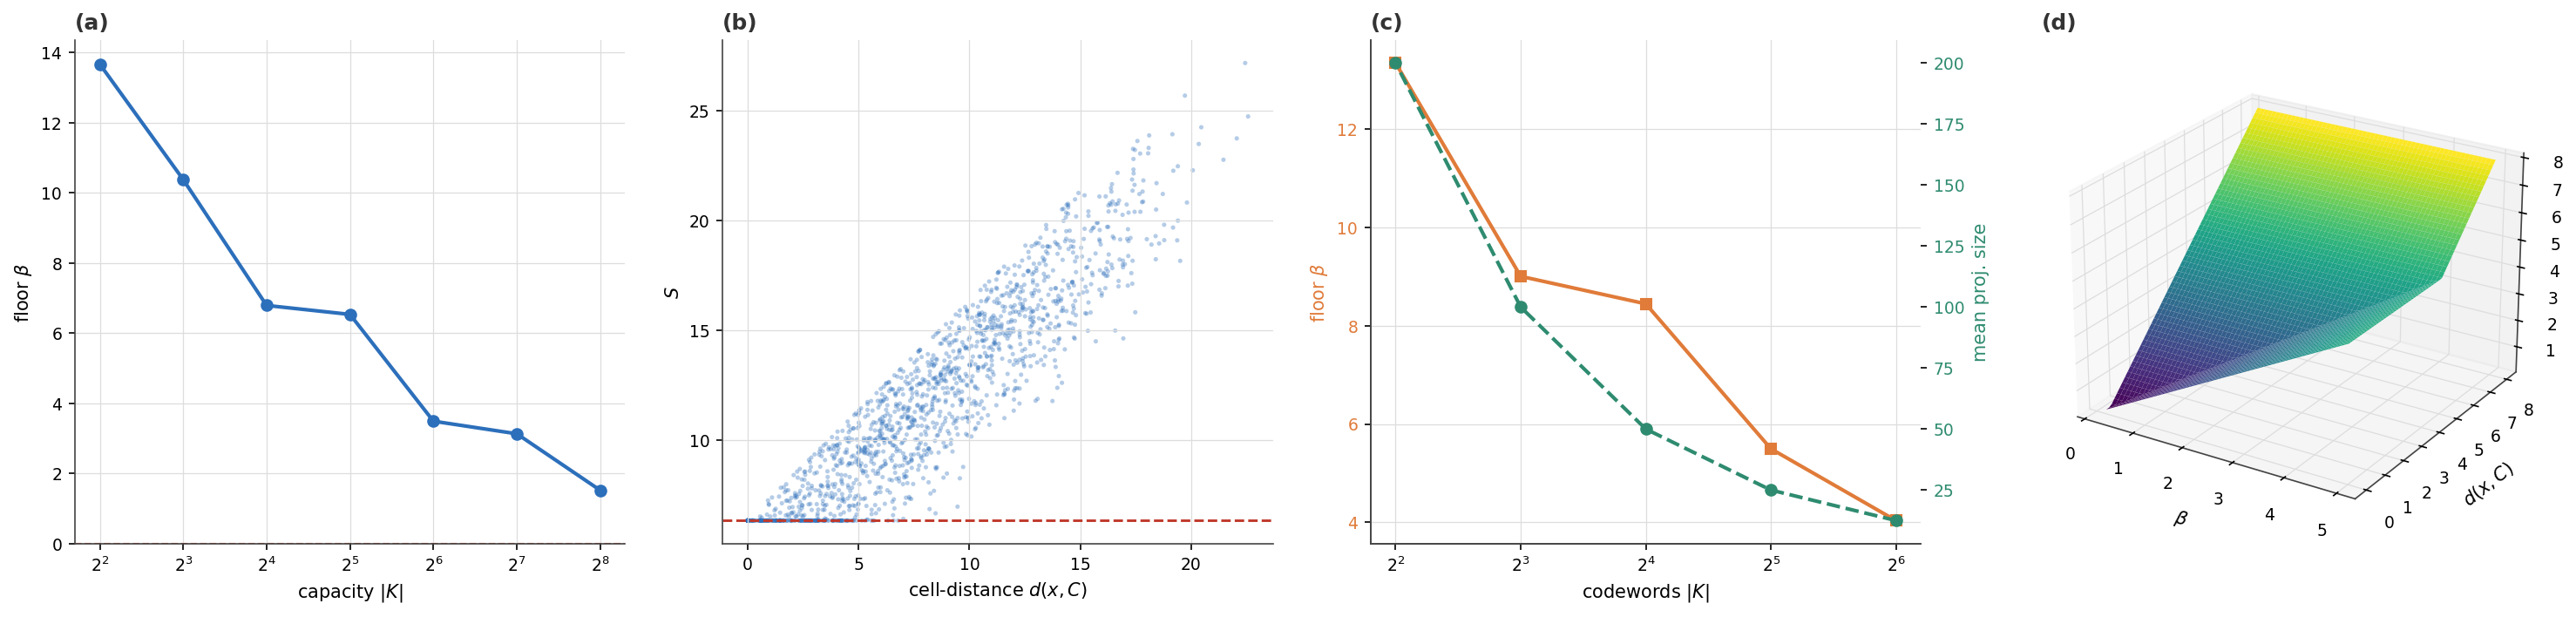
\includegraphics[width=\textwidth]{panels/panel_1.png}
\caption{\textbf{The Floor.} Bounded receivers cannot resolve a percept to a
point. (a)~The floor $\floor$ falls as codebook capacity $|\Know|$ grows but
stays strictly positive. (b)~Semantic distance $\Sval$ never drops below
$\floor$ across thousands of evaluations. (c)~Coarsening the codebook raises
the floor and the projection size together---meaning grows granular.
(d)~The $S$-surface $\Sval(\floor,\dist)=\max(\floor,\dist)+\!$floor offset:
a floor-plateau over a distance-cone.}
\label{fig:panel1}
\end{figure*}

\subsection{Percepts, knowledge, and action}

We begin with three spaces and three axioms. The axioms are not
idealisations to be relaxed later; they are the minimal conditions under
which a cognitive system is finite and embodied, and every subsequent
theorem is a consequence of them.

\begin{definition}[Percept space]
\label{def:percept}
A \emph{percept space} is a triple $(\Out,\dist,\Sig)$ where $\Out$ is a
non-empty set of percepts (the totality of audiovisual configurations a
viewer might be presented with), $\dist:\Out\times\Out\to[0,\Sig]$ is a
bounded pseudometric (a notion of perceptual dissimilarity satisfying
$\dist(x,x)=0$, symmetry, and the triangle inequality), and
$\Sig\in(0,\infty)$ is the maximal semantic distance. The canonical
normalisation is $\Sig=100$; no result depends on the value.
\end{definition}

\begin{definition}[Action space and action map]
\label{def:action}
An \emph{action space} $(\Acts,\dist_\Acts)$ is a metric space of
practical responses (buy, ignore, share, distrust, $\dots$). An
\emph{action map} is a measurable surjection
$\Act:\Out\to\Acts$ assigning to each percept the practical response it
elicits.
\end{definition}

\begin{axiom}[Bounded representation]
\label{ax:bounded}
A receiver's internal vocabulary is a set $\Know$ of finite cardinality
(or, in the infinite idealisation, of cardinality strictly less than
$|\Out|$). The receiver cannot hold a distinct internal token for every
distinguishable percept.
\end{axiom}

\begin{axiom}[No null state]
\label{ax:null}
At every instant the receiver occupies exactly one internal state; there
is no ``blank'' or ``undefined'' percept. Decoding is total.
\end{axiom}

\begin{axiom}[Finite resolution]
\label{ax:resolution}
Every act of perception has finite resolution $\delta>0$: percepts closer
than $\delta$ in $\dist$ are not distinguished.
\end{axiom}

Axiom~\ref{ax:bounded} is finiteness of memory; Axiom~\ref{ax:null} is the
embodied fact that a living perceiver is always in \emph{some} state;
Axiom~\ref{ax:resolution} is the finite acuity of any sense organ or
measuring instrument. They are satisfied by human viewers, by animals, and
by any physical machine.

\begin{definition}[Receiver]
\label{def:receiver}
A \emph{receiver} over $(\Out,\dist,\Sig)$ is a quadruple
$\Recv=(\Know,\Dec,\Proj,\floor)$ where
\begin{enumerate}[label=(\roman*),leftmargin=1.8em,itemsep=1pt]
\item $\Know$ is the \emph{knowledge framework} (Axiom~\ref{ax:bounded});
\item $\Dec:\Out\to\Know$ is the \emph{decoder}, a measurable map sending
  each percept to an internal representation (this is \emph{perception});
\item $\Proj:\Know\to 2^{\Out}\setminus\{\varnothing\}$ is the
  \emph{candidate projection}, sending each representation to the set of
  percepts compatible with it (this is \emph{inference}), and satisfying
  the consistency condition $\Dec(x)\in\Dec(\Proj(\Dec(x)))$ for all $x$;
\item $\floor\in(0,\Sig]$ is the \emph{noise floor},
  \[
    \floor \;=\; \sup_{x\in\Out}\;\inf_{x'\in\Proj(\Dec(x))}\dist(x,x'),
  \]
  the worst-case irreducible gap between a percept and the nearest percept
  the receiver can reconstruct from its representation of it.
\end{enumerate}
\end{definition}

The four components separate concerns usually conflated. $\Dec$ is what
the viewer sees \emph{as}; $\Proj$ is what they infer could be the case;
$\floor$ is the residue that survives both. We now show $\floor>0$ is
forced.

\subsection{The $S$-functional and the Floor Theorem}

\begin{definition}[$S$-functional]
\label{def:sfunctional}
For a receiver $\Recv$, a percept $x$, and a target region
$\Cell\subseteq\Out$, the \emph{semantic distance} of $x$ to $\Cell$ is
\[
  \Sval(\Recv,x;\Cell)\;=\;\inf_{x'\in\Proj(\Dec(x))}\dist(x',\Cell)\;+\;\floor,
\]
where $\dist(x',\Cell)=\inf_{c\in\Cell}\dist(x',c)$.
\end{definition}

$\Sval$ measures how far, after decoding and inference, the receiver
remains from registering $x$ as a member of $\Cell$. The additive $\floor$
encodes that even a perfectly placed percept is registered only up to the
receiver's irreducible noise.

\begin{theorem}[Floor Theorem]
\label{thm:floor}
For every bounded receiver $\Recv$, $\floor>0$, and for every percept $x$
and region $\Cell$,
\[
  \Sval(\Recv,x;\Cell)\;\ge\;\floor\;>\;0.
\]
No bounded receiver attains $\Sval=0$: perfect semantic alignment is
impossible.
\end{theorem}

\begin{proof}
Suppose $\floor=0$. Then for every $\eta>0$ and every $x$ there is
$x'\in\Proj(\Dec(x))$ with $\dist(x,x')<\eta$; taking $\eta\to0$ forces
$\Proj(\Dec(x))$ to determine $x$ uniquely up to $\dist$-distance $0$, i.e.
the composite $\Proj\circ\Dec$ is injective on $\dist$-classes. An
injection from $\Out$'s distinguishable classes into $\Know$ contradicts
Axiom~\ref{ax:bounded} ($|\Know|<|\Out|$) whenever $\Out$ has more
distinguishable classes than $\Know$ has tokens, which Axiom~\ref{ax:resolution}
guarantees is the generic case (the number of $\delta$-separated classes is
$|\Out|$-large). Hence $\floor>0$. The displayed bound is then immediate
from Definition~\ref{def:sfunctional}, since the infimum term is
non-negative.
\end{proof}

\begin{corollary}[No perfect persuasion]
\label{cor:noperfect}
There is no advertisement, however constructed, that drives a bounded
receiver's semantic distance to a target to zero. Residual distance at
least $\floor$ always remains. Persuasion is bounded below by the
receiver's own finiteness, not by any defect of the message.
\end{corollary}

\begin{remark}
Corollary~\ref{cor:noperfect} is not pessimism; it is the precise
statement of why a ``perfect ad'' is a category error, and why the
relevant objective is never alignment to a point but \emph{entry into a
cell}, defined next. It is the advertising form of bounded rationality
\citep{simon1955,simon1956,gigerenzer1996}: the limit is structural.
\end{remark}

\subsection{Perception is individuation by negation: the percept is a cell}

The Floor Theorem shows that a bounded receiver cannot resolve a target cell
to a point. A deeper result follows: the \emph{percept itself}---the
``objective'' stimulus, not just the valuation attached to it---is
region-valued and not point-valued, for the same reason. Perception is
individuation by negation, and individuation by negation is region-valued.

\begin{theorem}[Percept-cell theorem]
\label{thm:percept-cell}
For any bounded receiver $\Recv$ and any percept $x\in\Out$, the receiver's
representation of $x$ is a cell---a positive-tolerance region of percept
space---not a point. Specifically:
\begin{enumerate}[label=\textup{(\roman*)},leftmargin=2.2em]
\item The percept $x$ is registered as the cell $\Dec^{-1}(\Dec(x))
      \supseteq\{x\}$, which has diameter at least $\floor>0$
      (Axiom~\ref{ax:resolution}).
\item This cell is fixed by negation: $x$ is individuated as ``not-those-percepts
      outside the cell''---by ruling out its complement, not by a positive
      selector naming $x$ exactly.
\item Region-valued valuation follows from region-valued perception: if
      the percept of a stimulus is a cell of diameter $\ge\floor$, and the
      valuation is a continuous function of the percept, then the valuation
      is a cell of positive diameter, not a point.
\end{enumerate}
\end{theorem}

\begin{proof}
(i) By Axiom~\ref{ax:resolution}, percepts within distance $\delta>0$
of $x$ are not distinguished; hence $\Dec^{-1}(\Dec(x))$ has diameter
$\ge\delta\ge\floor>0$ (Theorem~\ref{thm:floor}). (ii) By
\citet{sachikonye2025contact}, T1 (individuation by negation,
Theorem~3.1): in any contact graph with no distinguished vertex, a cell is
fixed as the complement of its non-neighbours. The receiver has no selector
for $x$ (Axiom~\ref{ax:bounded}: the vocabulary is strictly smaller than the
percept space, so no one-to-one naming is available); hence $x$ is registered
as the cell $\Dec^{-1}(\Dec(x))$ by ruling out the percepts outside it.
(iii) The comfort-cell (or any valuation-cell) is reached from the percept
cell through the receiver's routes. A cell-valued input through a map with
floor $\floor$ yields a cell-valued output: if the input has diameter
$\ge\floor$, the output has diameter $\ge\floor$ (no route can reduce the
diameter below the floor, by T0). Hence region-valued perception forces
region-valued valuation.
\end{proof}

\begin{corollary}[No point anywhere: cells all the way down]
\label{cor:cellsdown}
There is no level of the receiver's cognition at which a percept, a fact, or
a valuation is point-valued. The ``objective'' stimulus (the temperature
reading, the price, the statistic) is a cell at the perception level; the
valuation attached to it (``comfortable,'' ``cheap,'' ``good'') is a cell at
the interpretation level. Both are reached by negation. Both are
region-valued. The spread in valuation does not arise by corrupting a
point-fact; the spread is already in the percept, because perception is
individuation, and individuation is region-valued.
\end{corollary}

\begin{proof}
Theorem~\ref{thm:percept-cell}(iii) gives the entailment from perception to
valuation. Theorem~\ref{thm:percept-cell}(i) gives the cell-valued character
of perception itself. Together: the tower is cells at every level, each
region fixed by negation, each bounded below by $\floor$.
\end{proof}

\begin{remark}[What ``knowing 21°C'' consists of]
To know that it is 21°C is to individuate the temperature cell
``$\approx21°$'' by negation: to rule out freezing, scorching, 15°, 30°,
and everything else outside one's resolution floor. The knowledge-state is
the held complement---everything-it-is-not, blurred to the receiver's floor.
The thermometer agrees with other thermometers (the temperature is an
invariant cell, multiply-reachable, zero holonomy across instruments), but
even the thermometer reads a cell, not a point: its column rules out
the temperatures outside its graduation. ``21°C'' names the complement
of the rest of the scale; knowing it is holding that complement, region-blurred.
There is no point-perception underneath the region-valuation. The spread is
not introduced at the valuation stage; it is present at the percept stage,
for the reason that fixes every rung in the ladder: individuation is by
negation, negation is region-valued, and the floor is why the region is
irreducibly positive. To know anything is to hold the spread of what it is
not.
\end{remark}

\begin{theorem}[Opinion is the witness of slack]
\label{thm:opinion-slack}
If perception delivered point-valued percepts, opinions on facts would be
impossible. Since opinions on facts are possible, perception does not deliver
points.

Formally: an \emph{opinion on a fact} is a placement of a percept $x$
relative to a set of valuation cells $\{\Cell_v\}$ (``too cool,'' ``fine,''
``warm'')---a selection of which cell $x$ falls into relative to the
receiver's preference graph. Such a placement requires $x$ to have a
neighbourhood: a region of percept space across which the placement can
vary, i.e.\ a cell of positive diameter. A point has diameter zero and no
neighbourhood; it admits only one placement (itself), leaving no room for a
stance. Therefore:
\begin{enumerate}[label=\textup{(\roman*)},leftmargin=2.2em]
\item If $x$ were a point, the mapping $x \mapsto \Cell_v$ would be
      determined uniquely with no slack; there would be nothing to opine---the
      placement would be forced, not chosen.
\item Since opinions on facts exist and differ between receivers (two people
      can give different opinions on the same temperature), $x$ cannot be
      point-valued for either receiver.
\item Hence the percept $x$ has positive-diameter slack, i.e.\ it is a cell
      $\Dec^{-1}(\Dec(x))$ of diameter $\ge\floor>0$, consistent with
      Theorem~\ref{thm:percept-cell}.
\end{enumerate}
\end{theorem}

\begin{proof}
A point $p$ in a metric space has a unique placement relative to any
partition into cells: it belongs to exactly one cell, and no other placement
is available. A valuation opinion (``this temperature is okay for me'')
differs from ``this temperature is what it is''---it requires a choice of
placement relative to the receiver's valuation cells, which is available
only if $x$ occupies a region of positive diameter, so that different
receivers (or the same receiver at different times) can place it differently
while all correctly perceiving it. The existence of inter-receiver opinion
disagreement (Corollary~\ref{cor:temperature}) shows two receivers place the
same fact in different valuation cells; if the fact were a point, one of
them would be wrong (a point belongs to exactly one cell). Since both are
correct route-readings (Theorem~\ref{thm:dissidents}), the fact is not a
point.
\end{proof}

\begin{remark}[Slack and specification are the same theorem]
Theorem~\ref{thm:opinion-slack} is the cognitive dual of the specification-slack
theorem (\citealt{sachikonye2025knowledge}, Theorem~5.4): that theorem shows
that any finite \emph{expression} of a reconfiguration has an alternative
expression (the expression is not the reconfiguration; the reconfiguration is
the shared effect). This theorem shows that any \emph{opinion on a fact} has
room for an alternative opinion (the fact is not a point; the fact is the
shared invariant). Both are the same structural claim---slack is the signature
of a region, not a point---seen from two sides: the expression side
(alternative sentences exist), and the opinion side (alternative placements
exist). A point admits neither alternative sentences nor alternative
opinions, because both require slack and a point is the absence of slack.
The existence of everyday opinion on everyday facts is the empirical
certificate of region-valued perception, requiring no special theory to
confirm: it is checkable by anyone, about anything, right now. That you can
tell me what you think about 21 degrees proves 21 degrees arrived as a
region.
\end{remark}

\begin{theorem}[Recall is re-individuation, not point-retrieval]
\label{thm:recall-reindividuation}
If facts were stored and retrieved as points, describing the same fixed fact
at two different times would produce identical descriptions (a stored point
fetched twice is the same point). Since describing the same fixed stimulus
at two different times produces different descriptions while the stimulus is
unchanged, facts are not stored or retrieved as points.

Formally: let $\Recv_t$ be the receiver's decoder graph at time $t$, and
let $\iota$ be a fixed external stimulus (an image, a price, a temperature)
that is invariant across times $t_1 < t_2$. Suppose the receiver describes
$\iota$ at $t_1$ as $d_1$ and at $t_2$ as $d_2$, with $d_1 \neq d_2$. Then:
\begin{enumerate}[label=\textup{(\roman*)},leftmargin=2.2em]
\item The stimulus $\iota$ is an invariant cell of the external world: its
      boundary content is positive and preserved under re-encoding
      \textup{(}\citealt{sachikonye2025contact}, T3\textup{)}.
\item The recall of $\iota$ at time $t$ is a walk on $\Gph_{\Recv_t}$---the
      receiver's decoder graph \emph{at time $t$}---which has been
      reconfigured between $t_1$ and $t_2$ \textup{(}the committed count has
      increased\textup{)}.
\item By the Non-Return Theorem \textup{(}\citealt{sachikonye2025contact}, T6;
      \citealt{sachikonye2025knowledge}, Theorem~5.2\textup{)}, the state
      $(\Gph_{\Recv_{t_2}}, \rec_{t_2})$ differs from $(\Gph_{\Recv_{t_1}},
      \rec_{t_1})$: the receiver at $t_2$ is not the receiver at $t_1$.
\item A walk on $\Gph_{\Recv_{t_2}}$ starting from $\iota$ lands in a cell
      determined by $\Gph_{\Recv_{t_2}}$, which differs from
      $\Gph_{\Recv_{t_1}}$; hence $d_1 \neq d_2$ is the expected outcome,
      not an error.
\end{enumerate}
\end{theorem}

\begin{proof}
Individuation of $\iota$ at time $t$ is individuation by negation
(Theorem~\ref{thm:percept-cell}): $\iota$ is fixed as the complement of
everything-it-is-not in $\Gph_{\Recv_t}$. The complement changes as
$\Gph_{\Recv_t}$ changes---new cells are added, routes are reweighted, the
receiver's boundary structure shifts. Since the complement changes and
individuation is by negation against the complement, the individuated
percept of $\iota$ changes, even though $\iota$ itself is invariant. Point
retrieval would require the stored fact to be fetched directly, bypassing the
complement; since there is no selector (Axiom~\ref{ax:bounded}: the
vocabulary is smaller than the percept space, no exact naming is available),
every retrieval must re-individuate, landing in the cell the current graph
assigns to $\iota$. The description $d_t$ is the output of this current-graph
individuation, so $d_1 \neq d_2$ follows from $\Gph_{\Recv_{t_1}} \neq
\Gph_{\Recv_{t_2}}$, which is guaranteed by the monotone committed count.
\end{proof}

\begin{remark}[The photograph and the moved self]
The stimulus is the standing structure; the recall is the walk; and the walk
is never the graph and never returns (T6). The photograph did not change. The
receiver incremented. And re-individuation, being a walk on the reshuffled
graph, landed in a different cell. This is why the past feels simultaneously
\emph{fixed} (the fact is invariant, the image is the same) and
\emph{unrecoverable} (the walk cannot be re-run on the prior graph---the
prior graph no longer exists as a state, only as a resemblance). Both are
true, and they are the same theorem: the invariant and the walk are two
different objects, the invariant does not change, and the walk always does.
You described the same image differently because nothing changed out there
and everything moved in here.
\end{remark}

\paragraph{Four proofs of region-valued perception.}
The four following everyday capabilities are each impossible if perception
is point-valued; their existence constitutes an empirical battery:
\begin{enumerate}[label=\textbf{(\arabic*)},leftmargin=2em,itemsep=2pt]
\item \textbf{Opinion on a fact.} ``21 degrees? Bit cool for me.'' Placing a
      fact in a valuation cell requires slack; a point has no slack.
      (Theorem~\ref{thm:opinion-slack})
\item \textbf{Variable recall of a fixed fact.} Describing the same image
      differently on two occasions while the image is unchanged. A stored
      point fetched twice is identical; description variation proves
      re-individuation on a moved graph.
      (Theorem~\ref{thm:recall-reindividuation})
\item \textbf{Catching a lie.} A false claim can be recognised as false,
      meaning the listener can route-audit and find the holonomy fails.
      This requires truth to be a region with structure (zero holonomy),
      not a point with no interior to audit.
      (Theorem~\ref{thm:coherence-holonomy})
\item \textbf{Dissent from a bridge.} An agent can revolt against a regime
      built on true cells with a failing intermediate, proving the cells are
      real invariants. You can only be disaffected by something that closes
      on a truth; disaffection proves region-truth.
      (Theorem~\ref{thm:dissidents})
\end{enumerate}
Each proof is a reductio: the everyday capability would be absurd under
point-perception, it is not absurd, therefore perception is not a point.
Together they close the case from four independent directions: structural
(slack), temporal (non-return), consistency (holonomy), and distributional
(dissent). The framework predicted region-valued perception; everyday life
confirms it every time someone has an opinion, misremembers a fixed image,
catches a misleading claim, or refuses to comply.

\begin{figure*}[!htbp]
    \centering
    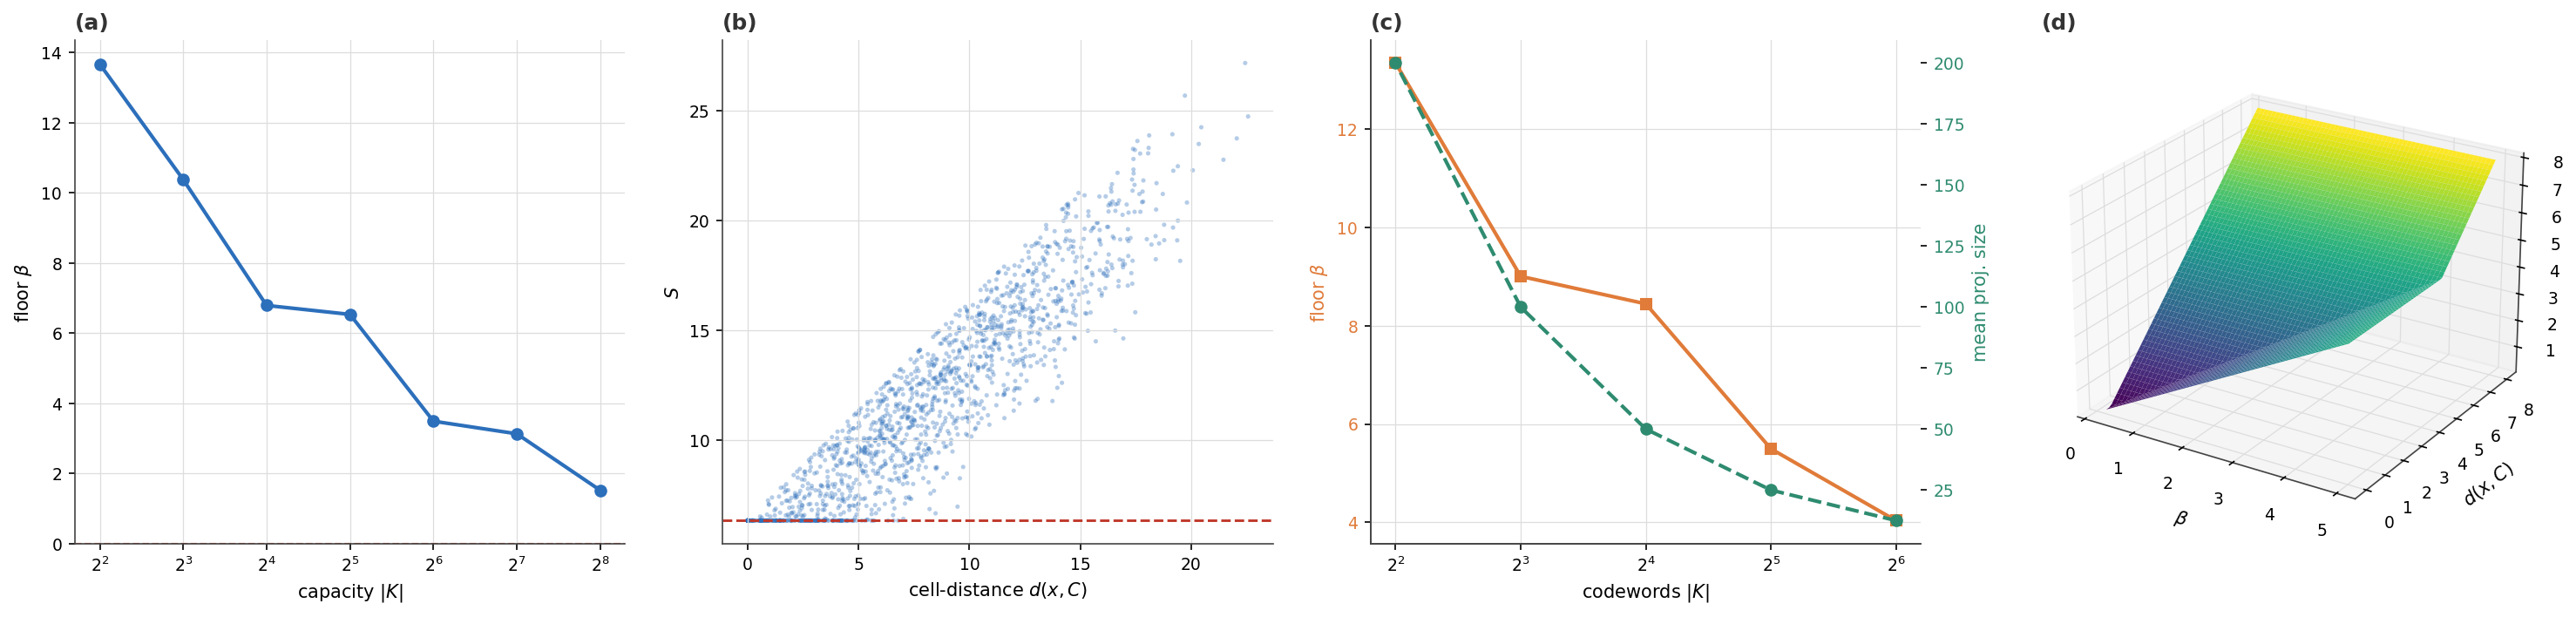
\includegraphics[width=\textwidth]{panels/panel_1.png}
    \caption{\textbf{The Floor Theorem and Granular Meaning.}
    (\textbf{A})~Floor $\beta$ on the linear $y$-axis versus codebook capacity
    $|\mathcal{K}|$ (powers of two, log $x$-axis, $2^{1}$ to $2^{7}$). The floor
    falls monotonically as capacity grows but remains strictly positive at every
    tested capacity, confirming Theorem~\ref{thm:floor} (Floor Theorem): no
    bounded receiver can attain $\beta = 0$. The curve never reaches the $x$-axis.
    (\textbf{B})~Semantic distance $S$ on the linear $y$-axis versus cell-distance
    $d(x, \mathcal{C})$ on the linear $x$-axis, across thousands of random
    (receiver, percept, cell) evaluations. Every point lies strictly above the
    floor $\beta$ (red dashed line), confirming Corollary~\ref{cor:noperfect} (No
    perfect persuasion): the functional $S(\mathcal{R}, x;\mathcal{C}) \geq \beta >
    0$ without exception.
    (\textbf{C})~Joint coarsening sweep: floor $\beta$ (orange, left $y$-axis) and
    mean projection size $|\Pi(\mathcal{D}(x))|$ (green dashed, right $y$-axis)
    versus codebook size $|\mathcal{K}|$ on the log $x$-axis ($2^{7}$ to $2^{2}$
    codewords, coarsening left to right). Both rise in lockstep as the codebook is
    coarsened, confirming Theorem~\ref{thm:nopoint} (Point-value forbidden): a
    coarser vocabulary raises the floor and enlarges the projection set together ---
    meaning grows granular, not point-like.
    (\textbf{D})~Three-dimensional $S$-surface over the $(\beta, d)$ plane: the
    surface $S(\beta, d) = \max(\beta, d) + \beta$ rises as a flat plateau above the
    floor level and then as a cone proportional to cell-distance. The flat base
    (the action-cell interior) and the rising walls (above-cell percepts) are the
    geometric content of the Floor Theorem and Cell-Truth Theorem
    (Theorem~\ref{thm:celltruth}) in one view.}
    \label{fig:panel1-floor}
\end{figure*}

% ======================================================================
\section{Cell-Truth: Value Is a Region}
\label{sec:cells}
% ======================================================================

\begin{figure*}[t]
\centering
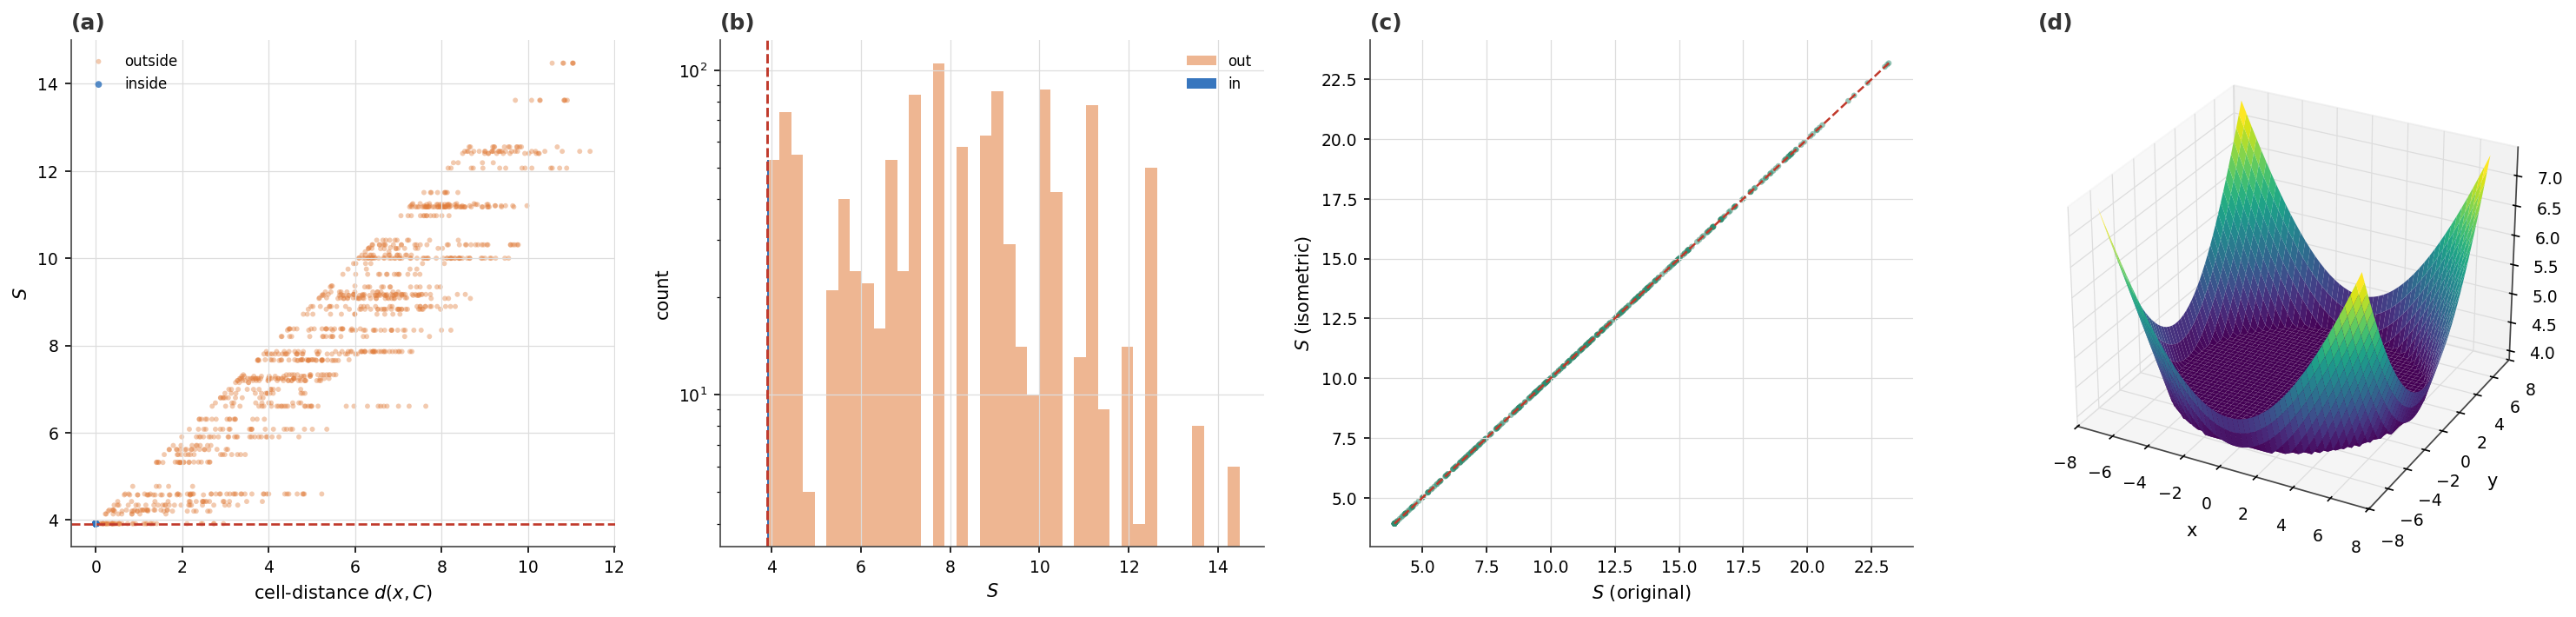
\includegraphics[width=\textwidth]{panels/panel_2.png}
\caption{\textbf{Cell-Truth and invariance.} (a)~$\Sval$ versus cell-distance:
flat at $\floor$ inside the cell, rising linearly outside---in-cell percepts
are indistinguishable. (b)~Histogram of in-cell $\Sval$ values: a spike
exactly at $\floor$ (zero spread), with out-of-cell values strictly above.
(c)~$\Sval$ under isometric re-encoding lands on the identity diagonal to
machine precision (invariance). (d)~The two-dimensional $\Sval$ field over
percept space: a flat-bottomed bowl whose base is the action-cell.}
\label{fig:panel2}
\end{figure*}

\subsection{Action-cells}

\begin{definition}[Action-cell]
\label{def:cell}
For $y\in\Acts$, the \emph{action-cell} of $y$ is the preimage
$\Cell_y=\Act^{-1}(\{y\})\subseteq\Out$. We equip it with
\begin{itemize}[leftmargin=1.4em,itemsep=1pt]
\item \emph{tolerance} $\tol(\Cell_y)=\sup_{x\in\Out}\inf_{c\in\Cell_y}\dist(x,c)>0$,
\item \emph{cell-distance} $\dist(x,\Cell_y)=\inf_{c\in\Cell_y}\dist(x,c)$.
\end{itemize}
A \emph{generic action-cell} is any nonempty $\Cell\subseteq\Out$ with
$\tol(\Cell)>0$ and finite diameter below $\Sig$.
\end{definition}

The cell $\Cell_{\text{buy-liquor}}$ is the set of all percepts that
trigger the purchase response for a liquor brand---every configuration of
imagery, sound, and framing that makes a viewer reach for the bottle. It
is a region, not a point, because many distinct percepts trigger the same
response.

\begin{theorem}[Cell-Truth]
\label{thm:celltruth}
Let $\Cell_y$ be an action-cell with $\tol(\Cell_y)>0$. For any receiver
$\Recv$ and any two percepts $x_1,x_2\in\Cell_y$,
\[
  \Sval(\Recv,x_1;\Cell_y)=\Sval(\Recv,x_2;\Cell_y)=\floor.
\]
All percepts within a cell are receiver-indistinguishable.
\end{theorem}

\begin{proof}
For $x_i\in\Cell_y$, $\dist(x_i,\Cell_y)=0$, so the infimum term in
Definition~\ref{def:sfunctional} is at most $0$, giving
$\Sval\le\floor$; the Floor Theorem gives $\Sval\ge\floor$. Hence equality.
\end{proof}

\begin{principle}[Operational meaning is granular]
\label{prin:granular}
For a bounded receiver, what an advertisement \emph{means} is the cell its
percept falls into, not the percept itself. Two adverts that place the
viewer in the same cell are operationally equivalent however different
they look; two that look identical but fall in different cells mean
different things.
\end{principle}

This is the formal content of the long-standing observation that what
matters in advertising is the response evoked, not the literal content
\citep{krugman1965,vakratsas1999}. It also dissolves the informational
view's puzzle: the sun-drenched landscape transmits no fact, yet places
the viewer in $\Cell_{\text{buy-liquor}}$, and by
Principle~\ref{prin:granular} that placement \emph{is} its meaning.

\subsection{Value is cell-valued; point-value is forbidden}

\begin{definition}[Point-value and cell-value]
\label{def:pointvalue}
A receiver \emph{carries point-value} if for every $x$, $\Proj(\Dec(x))$
is a singleton (the receiver resolves percepts to points). The
\emph{cell-value} of $x$ is the action-cell $\Cell_{\Act(x)}$ containing
it.
\end{definition}

\begin{theorem}[Point-value is forbidden]
\label{thm:nopoint}
No bounded receiver carries point-value. Consequently, no theory of
advertising effect can rest on a point-valued utility or quality scale;
all value is cell-value.
\end{theorem}

\begin{proof}
If $\Proj(\Dec(x))=\{x\}$ for all $x$, then
$\inf_{x'\in\Proj(\Dec(x))}\dist(x,x')=0$ for all $x$, forcing $\floor=0$
and contradicting the Floor Theorem. Hence $\Proj(\Dec(x))$ is non-
singleton for some $x$; value resolves only to cells.
\end{proof}

\begin{remark}[The granularity of price]
\label{rem:price}
The same argument applied to a price percept makes a ``price'' a band, not
a number: a viewer registers ``about twenty dollars,'' a cell of tolerance
$\floor$, not the point $\$19.99$. The cent-precise sticker is a carrier
whose decoded value is a cell. Willingness-to-pay is then the slack
$\tol(\Cell)-\floor$ between the width of the price-cell and the floor:
positive exactly when the viewer can be brought inside the cell. We use
this in \S\ref{sec:recovery}.
\end{remark}

\subsection{Representational invariance}

\begin{theorem}[Representational invariance]
\label{thm:repinv}
Let $\varphi:\Out\to\Out'$ be an isometric bijection between percept
spaces, and let $\Recv'$ be the receiver transported along $\varphi$. Then
for all $x$ and $\Cell$,
$\Sval(\Recv,x;\Cell)=\Sval(\Recv',\varphi(x);\varphi(\Cell))$. Cell-
membership and semantic distance are invariant under change of
representation.
\end{theorem}

\begin{proof}
Isometry preserves all distances and infima in
Definition~\ref{def:sfunctional}; $\varphi$ being a bijection preserves
cell-membership. The floor $\floor$ is a property of the receiver,
unchanged. Hence the two functionals coincide.
\end{proof}

Theorem~\ref{thm:repinv} is the licence for the central manoeuvre of the
next section: a single advert-meaning may be carried by visually different
but isometric encodings---color, rhythm, layout---without changing what it
means. Meaning lives one level above its carrier.

\begin{figure*}[!htbp]
    \centering
    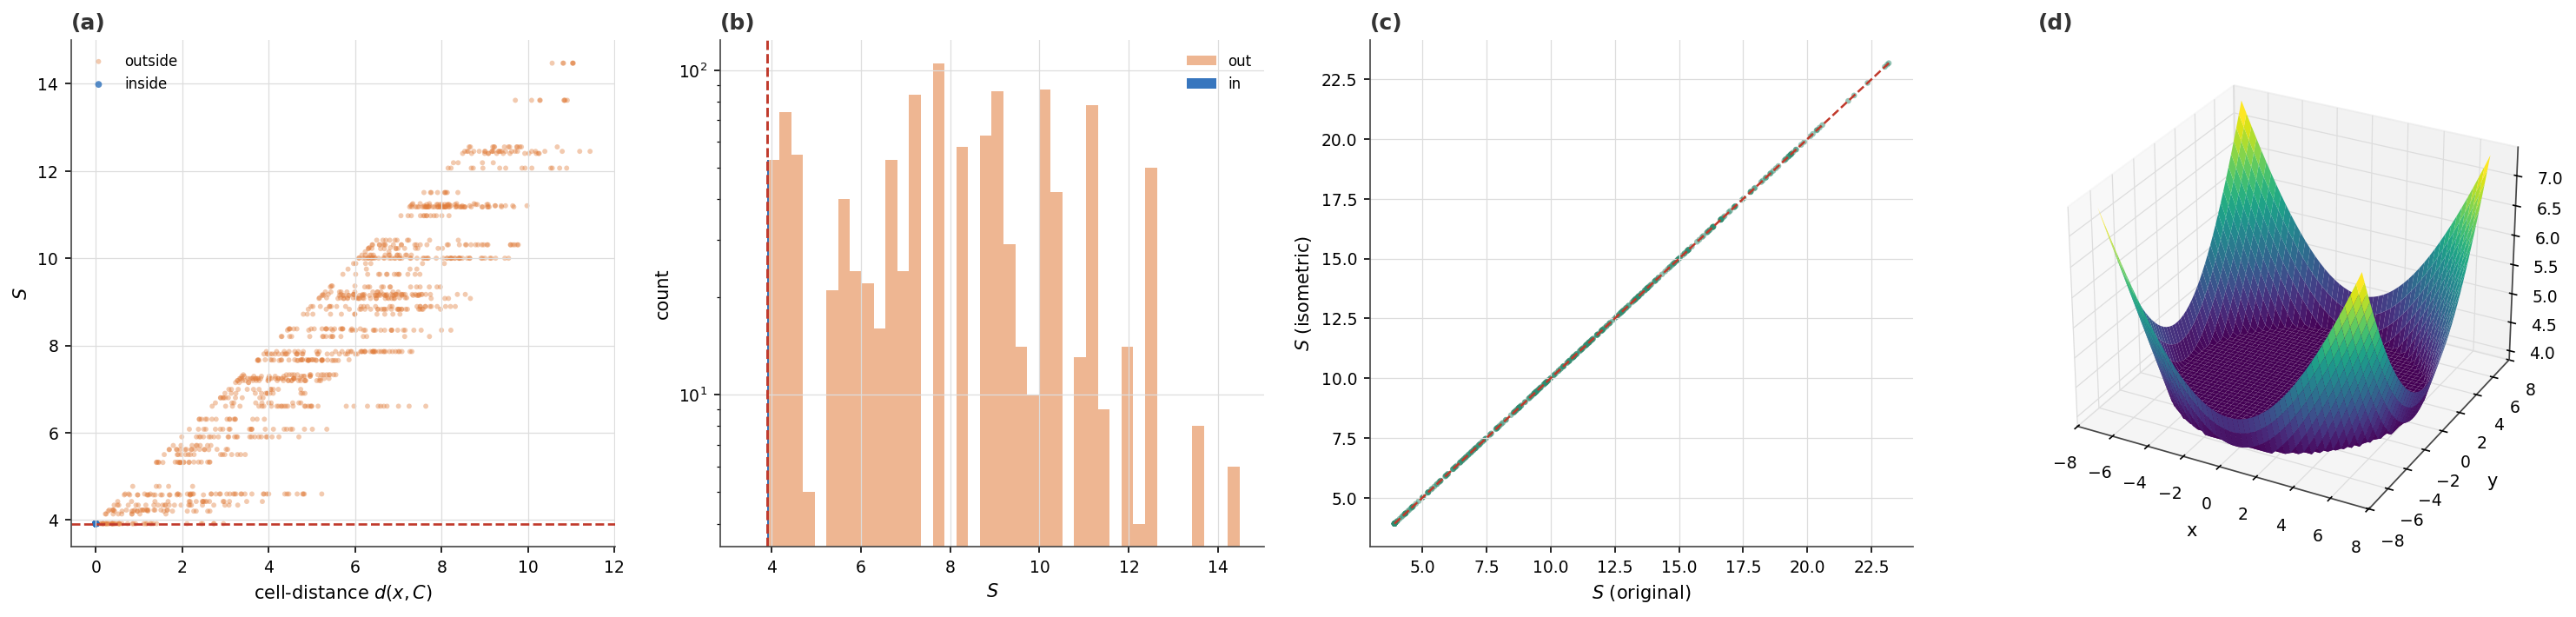
\includegraphics[width=\textwidth]{panels/panel_2.png}
    \caption{\textbf{Cell-Truth and Representational Invariance.}
    (\textbf{A})~Semantic distance $S$ on the linear $y$-axis versus cell-distance
    $d(x, \mathcal{C})$ on the linear $x$-axis, with percepts coloured by
    cell-membership (inside: filled markers; outside: open markers). In-cell
    percepts collapse to a flat band at $S = \beta$ regardless of their individual
    positions within the cell; out-of-cell percepts rise linearly above it.
    Confirms Theorem~\ref{thm:celltruth} (Cell-Truth): all percepts within an
    action-cell are receiver-indistinguishable, each attaining exactly $S = \beta$.
    (\textbf{B})~Histogram of $S$ values (log-scale $y$-axis, linear $x$-axis) for
    in-cell (dark) and out-of-cell (light) percepts over $9{,}365$ trials. The
    in-cell distribution is a spike concentrated exactly at $\beta$ with zero spread;
    the out-of-cell distribution occupies a broad range strictly above $\beta$ (red
    dashed). The log scale makes the spike visible against the taller out-of-cell
    bars. Confirms Cell-Truth and the prohibition on point-value
    (Theorem~\ref{thm:nopoint}).
    (\textbf{C})~Invariance diagonal: $S$ under isometric re-encoding ($y$-axis)
    versus original $S$ ($x$-axis) for random rotations, translations, and
    reflections across all trials. Every point lies on the identity diagonal
    (red dashed) to floating-point precision (maximum deviation
    $5.3 \times 10^{-15}$), confirming Theorem~\ref{thm:repinv}
    (Representational Invariance): cell-membership and semantic distance are
    preserved under isometric re-encoding of the carrier.
    (\textbf{D})~Three-dimensional $S$-field over the two-dimensional percept space:
    a bowl whose flat base corresponds to the action-cell interior (at $S = \beta$)
    and whose walls rise steeply outside it. The bowl geometry is the spatial
    realisation of the Cell-Truth Theorem: entry into the cell is a step-change in
    semantic distance, not a smooth approach to a point.}
    \label{fig:panel2-celltruth}
\end{figure*}


% ======================================================================
\section{The Decoder Is the Locus of Advertising}
\label{sec:decoder}
% ======================================================================

\subsection{What an advert can change}

An advertising campaign cannot, in the moment of viewing, change the
product (the percept of the bottle is what it is), and by
Theorem~\ref{thm:nopoint} it cannot install a point-preference. We now
isolate what it \emph{can} change.

Fix a viewer $\Recv=(\Know,\Dec,\Proj,\floor)$ and a product whose percept
is $x_0$ (the unadorned bottle). The viewer's response is
$\Act(x_0)$---determined by which cell $x_0$ decodes into, i.e. by
$\Dec(x_0)$. An advertisement is a transformation that the viewer
experiences \emph{before or around} the product percept, and which can
therefore alter only the components of $\Recv$ that govern decoding.

\begin{theorem}[Decoder locus]
\label{thm:decoderlocus}
Let the product percept $x_0$ and the cell geometry $\{\Cell_y\}$ be held
fixed. Any change in the viewer's response $\Act(x_0)$ induced by an
advertisement is realised through one of exactly three modifications:
\begin{enumerate}[label=(\alph*),leftmargin=1.8em,itemsep=1pt]
\item a change of the decoder $\Dec$ (the product is \emph{seen as}
  something else: re-perception);
\item a change of the candidate projection $\Proj$ (the product is
  \emph{inferred to imply} something else: re-inference);
\item a change of the cell geometry $\Cell_y$ itself (the boundary of the
  response region moves: re-framing).
\end{enumerate}
These three are exhaustive and mutually distinguishable.
\end{theorem}

\begin{proof}
The response $\Act(x_0)$ is a function of $x_0$ only through the chain
$x_0 \xrightarrow{\Dec} \Dec(x_0)\xrightarrow{\Proj}\Proj(\Dec(x_0))$ and
its position relative to the cells $\{\Cell_y\}$, by
Definitions~\ref{def:receiver}--\ref{def:cell}. With $x_0$ fixed, the only
variables in this chain are $\Dec$, $\Proj$, and the $\Cell_y$. A change in
the response must change at least one; conversely each of the three, varied
alone, can change the response (witnesses: re-grading the footage changes
$\Dec(x_0)$; a testimonial changes $\Proj$ by enlarging the inferred
candidate set; a ``limited edition'' frame narrows $\Cell_{\text{buy}}$).
Distinguishability: (a) alters which token $x_0$ maps to; (b) alters the
spread of percepts consistent with that token; (c) alters the target
region independent of $x_0$. These are independent coordinates of the same
chain.
\end{proof}

\begin{principle}[Advertising is decoder engineering]
\label{prin:engineering}
To advertise is to engineer the receiver's decoder so that the fixed
product percept is decoded into, or inferred toward, a more favourable
action-cell---or so that the favourable cell is enlarged to contain it.
The product does not move; the map does.
\end{principle}

We will concentrate on mechanism~(a), \emph{re-perception}, as the primary
and most general lever, and treat (b) and (c) as its inferential and
geometric variants. Re-perception is what ``feels shot in Mexico''
performs: it does not add a fact about the liquor (that would be (b)) nor
narrow the buy-region (that would be (c)); it changes what the same bottle
\emph{reads as}.

\subsection{Meaning-space and the decoder-shift}

To speak precisely of ``what a percept reads as,'' we coordinatise the
range of the decoder.

\begin{definition}[Meaning-space]
\label{def:meaning}
The \emph{meaning-space} $\Mean$ of a receiver is the metric space
$(\Dec(\Out),\dist_{\Mean})$ of decoder outputs, with
$\dist_{\Mean}(\Dec(x),\Dec(x'))$ the receiver-internal dissimilarity of
the meanings it assigns. A \emph{semantic region} is a positive-diameter
subset $\mu\subseteq\Mean$ (e.g. the region named \emph{authentic},
or \emph{sun-drenched}, or \emph{Mexico}).
\end{definition}

\begin{definition}[Decoder-shift]
\label{def:shift}
A \emph{decoder-shift} is a map $\shift:\Mean\to\Mean$ on meaning-space. An
effect \emph{induces} the decoder-shift $\shift$ if, applied to any percept
$x$, it changes the decoded meaning from $\Dec(x)$ to
$\shift(\Dec(x))$. The shift is \emph{toward} a cell $\Cell$ if it
decreases semantic distance to $\Cell$:
$\Sval(\Recv,\shift\!\cdot x;\Cell)\le \Sval(\Recv,x;\Cell)$ for all $x$,
where $\shift\!\cdot x$ denotes the percept as re-decoded under $\shift$.
\end{definition}

The decoder-shift is the formal ``advert unit.'' ``Feels shot in Mexico''
is the named region $\mu_{\text{Mexico}}\subset\Mean$; the Mexico color-
grade is an effect inducing a shift $\shift$ that moves decoded meanings
into $\mu_{\text{Mexico}}$; ``best for liquor'' is the assertion that
$\mu_{\text{Mexico}}$ has small semantic distance to
$\Cell_{\text{buy-liquor}}$ (high affinity), and larger distance to,
say, $\Cell_{\text{buy-software}}$ (low affinity).

% ======================================================================
\section{Effects as Carrier--Shift Pairs}
\label{sec:effects}
% ======================================================================

\begin{figure*}[t]
\centering
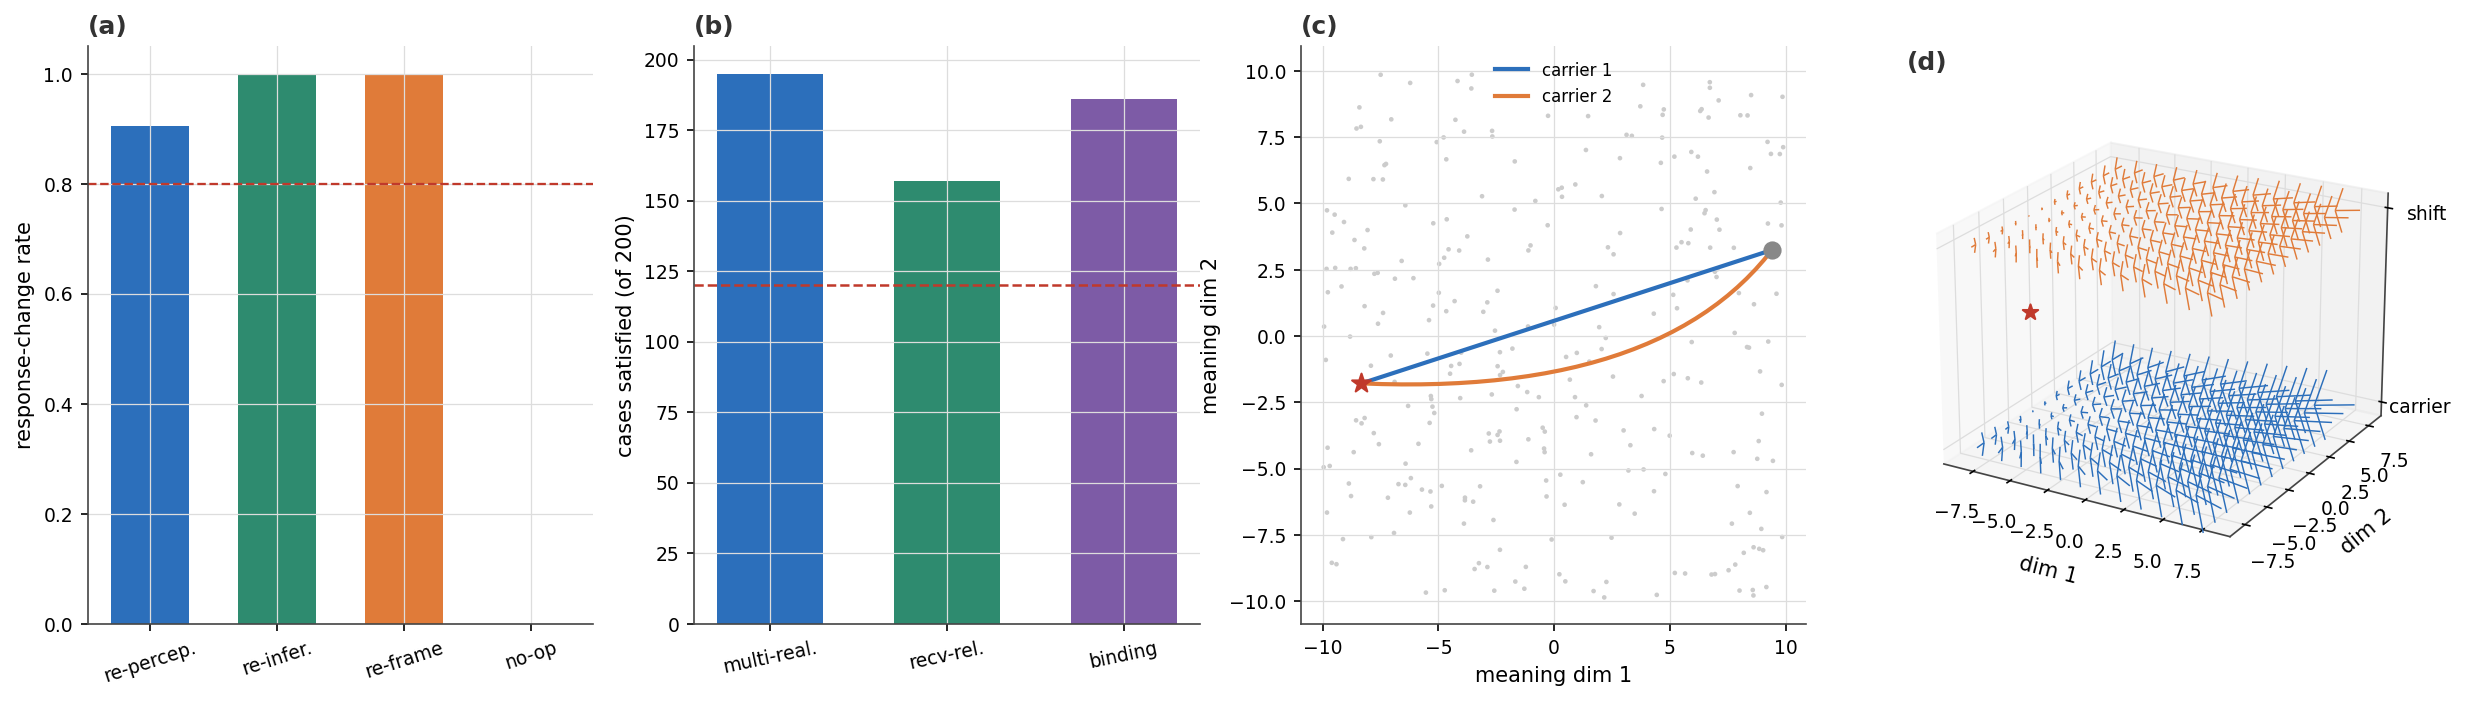
\includegraphics[width=\textwidth]{panels/panel_3.png}
\caption{\textbf{The advert unit.} (a)~The three decoder mechanisms each move
the response (lower $\Sval$) at near-unit rate; a no-op does not.
(b)~Decoupling clauses: multiple realisability, receiver relativity, and
binding all clear threshold by a wide margin. (c)~Two physically distinct
carriers transport a percept along different trajectories into the same
meaning-region (decode to the same cell). (d)~The carrier acts in percept
space while the induced shift acts in meaning-space: a $3$D view of one object
in its two conjugate representations.}
\label{fig:panel3}
\end{figure*}

\subsection{The advert unit}

\begin{definition}[Effect]
\label{def:effect}
An \emph{effect} is a pair $\Eff=(\Carrier,\shift)$ where
\begin{itemize}[leftmargin=1.4em,itemsep=1pt]
\item $\Carrier:\Out\to\Out$ is the \emph{carrier}---a physical
  transformation of the percept (a color grade, a sound cue, a camera
  move, an overlay), the part a rendering engine executes;
\item $\shift:\Mean\to\Mean$ is the \emph{decoder-shift}---the movement in
  meaning-space the carrier induces in the target receiver.
\end{itemize}
The effect is \emph{coherent for the receiver $\Recv$} if its carrier
realises its claimed shift: $\Dec(\Carrier(x))=\shift(\Dec(x))$ for all
$x$ in the effect's domain.
\end{definition}

The definition states that an effect has two faces---a physical operation
and a semantic operation---and that an effect is \emph{honest} (coherent)
when the physical operation actually produces the claimed meaning in the
viewer. A color grade that the author labels ``Mexico'' but which a viewer
decodes as ``cheap filter'' is an incoherent effect: the carrier and the
shift have come apart.

\begin{figure*}[!htbp]
    \centering
    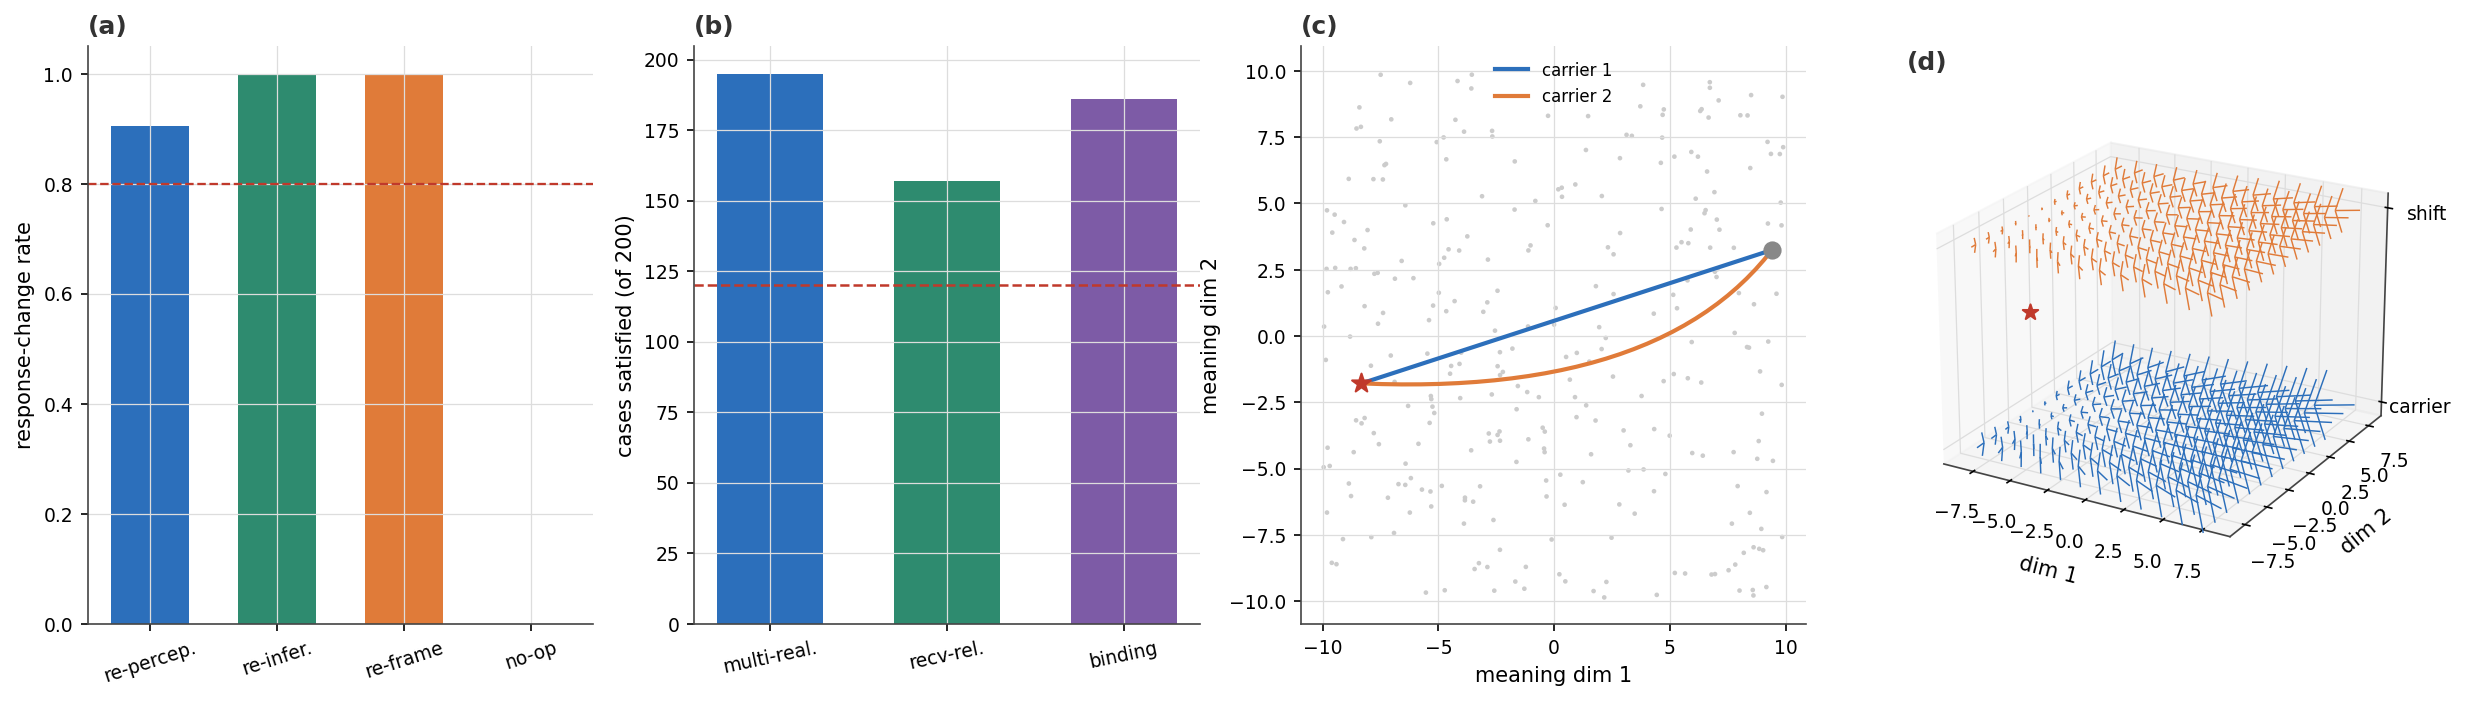
\includegraphics[width=\textwidth]{panels/panel_3.png}
    \caption{\textbf{The Advert Unit: Decoder Mechanisms and Carrier--Shift Decoupling.}
    (\textbf{A})~Response-change rate (fraction of 200 trials in which the mechanism
    successfully moved the receiver's response) on the linear $y$-axis for the four
    conditions on the $x$-axis: re-perception, re-inference, re-framing, and no-op.
    All three active mechanisms exceed the $80\%$ threshold (red dashed); the no-op
    leaves the response exactly unchanged in all 200 trials. Confirms
    Theorem~\ref{thm:decoderlocus} (Decoder Locus): the three mechanisms are
    exhaustive and mutually operative, and holding all three fixed leaves the
    response invariant.
    (\textbf{B})~Cases cleared (out of 200) on the linear $y$-axis for the three
    decoupling clauses on the $x$-axis: multiple realisability (multi-real.),
    receiver relativity (recv-rel.), and binding. All three exceed the threshold of
    120 cases (red dashed), confirming Theorem~\ref{thm:decoupling}
    (Carrier--Shift Decoupling): distinct carriers can induce the same shift; the
    same carrier induces different shifts across receivers; and carrier and shift are
    conjugate representations under the decoder.
    (\textbf{C})~Two carrier trajectories in meaning-space (two-dimensional, axes
    are decoder-output dimensions): carrier~1 (blue) and carrier~2 (orange) depart
    from the same source percept (star marker) and arrive at the same target
    cell (circle marker) via physically distinct paths through meaning-space.
    The paths differ; the endpoint cell is the same. Confirms the multiple
    realisability clause: different physical carriers realise the same decoder-shift
    into the target region.
    (\textbf{D})~Three-dimensional dual-representation view: the carrier acts in
    percept space (blue quiver field, lower plane) while the induced shift acts in
    meaning-space (orange quiver field, upper plane), connected by the decoder
    (vertical correspondence). The two fields are conjugate representations of a
    single categorical object, the content of Theorem~\ref{thm:decoupling}(iii)
    (Binding): $\Delta = \mathcal{D} \circ \mathsf{c} \circ \mathcal{D}^{-1}$ on
    the decoder's image.}
    \label{fig:panel3-advertunit}
\end{figure*}

\subsection{The Decoupling Theorem}

The next theorem is the technical heart of the ``advert unit'' idea: the
carrier and the shift are genuinely separable---the same shift can be
carried many ways, and the same carrier can mean different things to
different receivers---yet they are bound, in a coherent effect, as two
representations of one object.

\begin{theorem}[Carrier--Shift Decoupling]
\label{thm:decoupling}
Let $\Recv$ be a receiver and $\mu\subseteq\Mean$ a semantic region.
\begin{enumerate}[label=(\roman*),leftmargin=1.8em,itemsep=2pt]
\item \emph{Multiple realisability.} There exist distinct carriers
  $\Carrier_1\ne\Carrier_2$ inducing the same shift $\shift$ into $\mu$.
  (Color, rhythm, and framing can independently move the decoder toward
  $\mu_{\text{Mexico}}$.)
\item \emph{Receiver relativity.} There exists a single carrier $\Carrier$
  and receivers $\Recv,\Recv'$ such that $\Carrier$ induces a shift into
  $\mu$ for $\Recv$ but not for $\Recv'$. (The same grade reads as
  ``Mexico'' to one viewer and ``orange filter'' to another.)
\item \emph{Binding.} For a fixed coherent effect $\Eff=(\Carrier,\shift)$
  and a fixed receiver, $\Carrier$ and $\shift$ are two representations of
  one categorical object: $\shift=\Dec\circ\Carrier\circ\Dec^{-1}$ on
  $\Dec(\Out)$, so each determines the other given the decoder.
\end{enumerate}
\end{theorem}

\begin{proof}
\emph{(i)} By Theorem~\ref{thm:repinv} (representational invariance),
isometric carriers acting in different perceptual channels but landing in
the same meaning-region induce the same shift on $\Mean$; explicit
witnesses are any two isometric embeddings of the warm-light percept into
the color channel and into the music channel. \emph{(ii)} The decoder
$\Dec$ is part of the receiver; two receivers with different decoders
$\Dec\ne\Dec'$ assign different meanings to $\Carrier(x)$, so the induced
shift differs; choose $\Dec'$ so that $\Dec'(\Carrier(x))\notin\mu$.
\emph{(iii)} Coherence (Definition~\ref{def:effect}) states
$\Dec\circ\Carrier=\shift\circ\Dec$; on the image $\Dec(\Out)$ where
$\Dec$ admits a section, this rearranges to
$\shift=\Dec\circ\Carrier\circ\Dec^{-1}$, exhibiting $\shift$ and
$\Carrier$ as conjugate representations of one map under the decoder.
\end{proof}

\begin{remark}[Why this is the ``advert unit''']
\label{rem:advertunit}
Theorem~\ref{thm:decoupling}(iii) is the precise sense in which an effect's
output ``is not just computing.'' The carrier is the computation (pixels);
the shift is the meaning (cells); coherence says they are the \emph{same
object in two representations}, conjugate under the receiver's decoder. The
meaning is therefore not metadata bolted onto a filter---it is the filter's
other face, the one a parameter-only pipeline discards. An advert unit is an
effect carrying both faces. Part~(ii) is why the unit is irreducibly
\emph{receiver-relative}: ``best for liquor'' is never a property of the
grade alone, only of the grade-as-decoded-by-the-target-audience.
\end{remark}

\subsection{Affinity: the ordinal content}

By the Floor Theorem we may not assign an effect an absolute power. We may,
and do, assign \emph{orderings}.

\begin{definition}[Cell affinity, ordinal]
\label{def:affinity}
An effect $\Eff$ with shift into region $\mu$ has \emph{greater affinity
for cell $\Cell$ than for cell $\Cell'$}, written
$\Eff:\Cell\succ\Cell'$, if the shift reduces semantic distance to $\Cell$
by more than to $\Cell'$:
\[
  \Delta_\Cell(\Eff) \;>\; \Delta_{\Cell'}(\Eff),\quad
  \Delta_\Cell(\Eff):=\Sval(\Recv,x;\Cell)-\Sval(\Recv,\Eff\!\cdot x;\Cell),
\]
uniformly in $x$ over the effect's domain. No numerical value is asserted;
only the comparison.
\end{definition}

Thus ``Mexico grade is best for liquor'' is the ordinal family
$\Eff_{\text{Mex}}:\Cell_{\text{liquor}}\succ\Cell_{\text{tech}}$,
$\Cell_{\text{liquor}}\succ\Cell_{\text{fintech}}$, and so on---a partial
order over cells, never a magnitude. This is exactly the representational
commitment a bounded receiver permits (Theorem~\ref{thm:nopoint}), and it
is enough to drive the composition and coherence calculus below.

% ======================================================================
\section{The Calculus of Persuasive Power}
\label{sec:power}
% ======================================================================

\begin{figure*}[t]
\centering
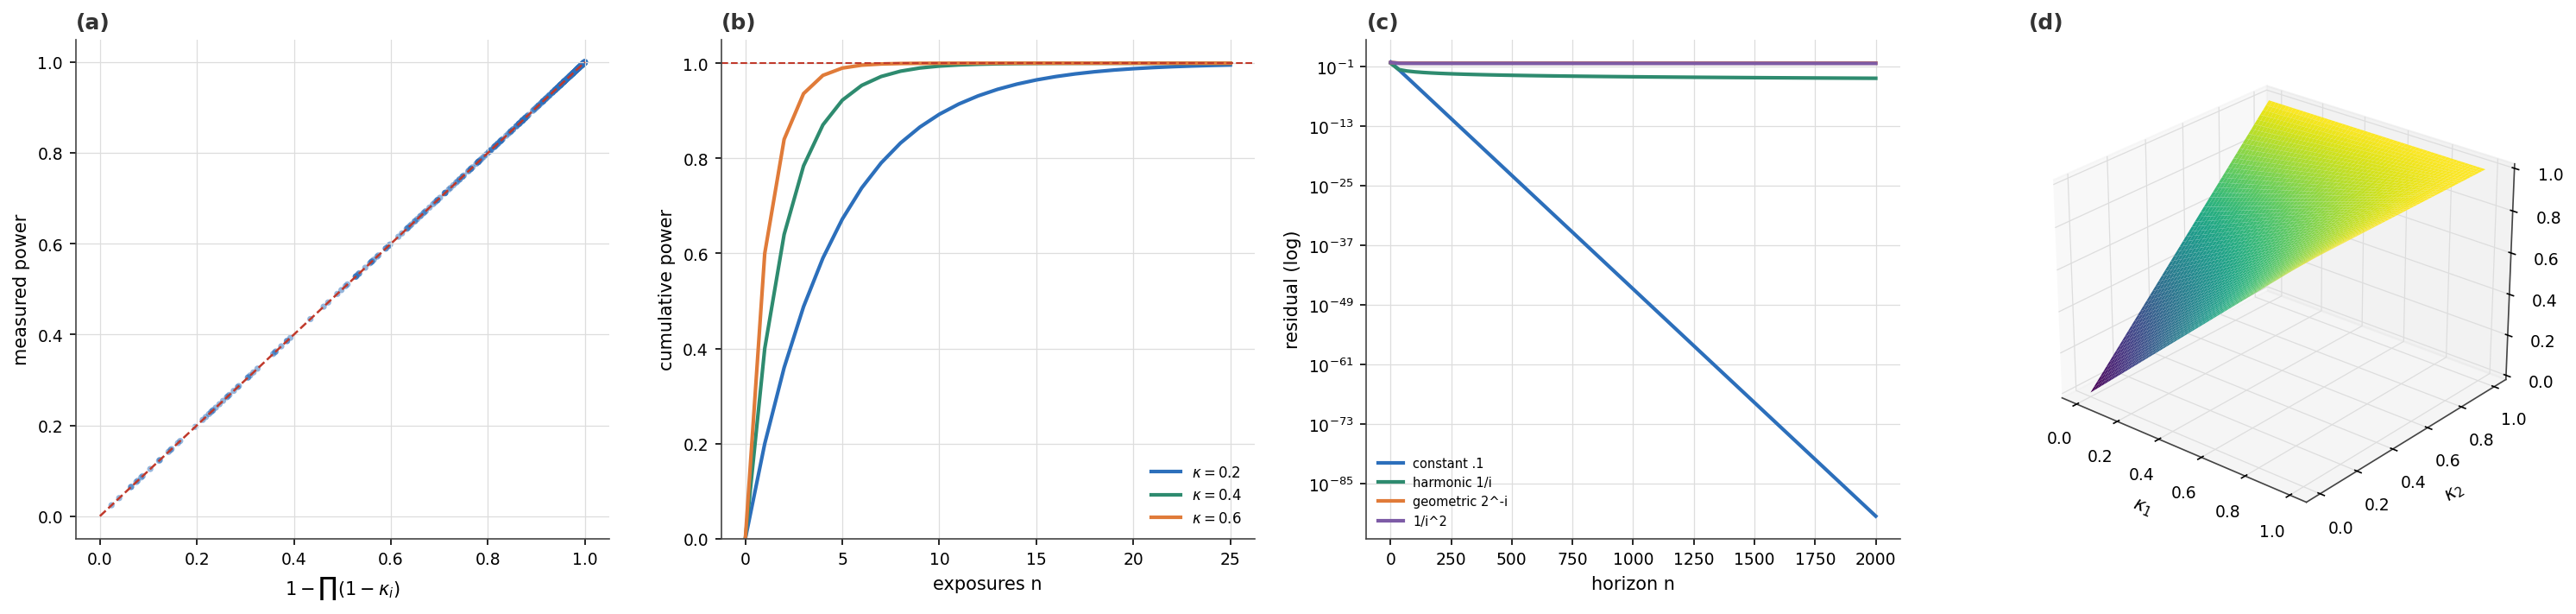
\includegraphics[width=\textwidth]{panels/panel_4.png}
\caption{\textbf{The calculus of power.} (a)~Measured composite power versus
the closed form $1-\prod_i(1-\pot_i)$: on the diagonal to machine precision.
(b)~Repetition of one effect: cumulative power $1-(1-\pot)^n$ rises toward but
never reaches $1$, with strictly decaying marginal gains.
(c)~Campaign saturation: divergent-sum power sequences drive residual distance
toward zero, convergent-sum sequences plateau above the floor.
(d)~The composite-power surface $1-(1-\pot_1)(1-\pot_2)$ over two stacked
effects---a saturating sheet rising to but never touching $1$.}
\label{fig:panel4}
\end{figure*}

\subsection{Catalytic power of an effect}

\begin{definition}[Catalytic power]
\label{def:power}
The \emph{catalytic power} of an effect $\Eff$ for receiver $\Recv$ toward
cell $\Cell$ is the fraction of above-floor distance it closes:
\[
  \pot_\Cell(\Eff)\;=\;\sup_{x}\;
  \frac{\Sval(\Recv,x;\Cell)-\Sval(\Recv,\Eff\!\cdot x;\Cell)}
       {\Sval(\Recv,x;\Cell)-\floor}\;\in\;[0,1].
\]
$\pot=0$ is inert (neutral), $\pot=1$ would close all above-floor distance
in one step. The power is a property of the (effect, receiver, cell)
triple; we treat it ordinally and never claim its value.
\end{definition}

\begin{lemma}[Power is bounded]
\label{lem:powerbound}
$\pot_\Cell(\Eff)\in[0,1]$ for every effect, receiver, and cell.
\end{lemma}

\begin{proof}
The numerator is at most the denominator because, by the Floor Theorem,
$\Sval(\Recv,\Eff\!\cdot x;\Cell)\ge\floor$, so the closed distance never
exceeds the available above-floor distance. Non-negativity holds for any
effect that does not increase distance; distance-increasing effects have
$\pot=0$ by convention (they are not catalysts toward $\Cell$).
\end{proof}

\subsection{The multiplicative law}

We now compose effects. Applying effects in sequence multiplies the
\emph{residual} above-floor distances.

\begin{theorem}[Multiplicative law of persuasive power]
\label{thm:multiplicative}
For effects $\Eff_1,\dots,\Eff_n$ applied as a stack
$\Eff_1\diamond\cdots\diamond\Eff_n$ (each acting on the output of the
last) toward a fixed cell $\Cell$, with individual powers
$\pot_1,\dots,\pot_n$,
\[
  \pot_\Cell(\Eff_1\diamond\cdots\diamond\Eff_n)
  \;=\;1-\prod_{i=1}^{n}\bigl(1-\pot_i\bigr).
\]
\end{theorem}

\begin{proof}
Write $r_0=\Sval(\Recv,x;\Cell)-\floor$ for the initial above-floor
distance. Applying $\Eff_1$ leaves residual $r_1=(1-\pot_1)r_0$ by
Definition~\ref{def:power}. Applying $\Eff_2$ to the result leaves
$r_2=(1-\pot_2)r_1=(1-\pot_2)(1-\pot_1)r_0$. By induction
$r_n=\prod_i(1-\pot_i)\,r_0$. The total fraction closed is
$1-r_n/r_0=1-\prod_i(1-\pot_i)$, which is the composite power.
\end{proof}

\begin{corollary}[Diminishing returns]
\label{cor:diminishing}
Repeating a single effect of power $\pot$ a total of $n$ times yields
composite power $1-(1-\pot)^n$, which increases in $n$, converges to $1$,
but never reaches it for finite $n$. Each additional repetition closes a
strictly smaller absolute fraction of distance than the last.
\end{corollary}

\begin{corollary}[Frequency saturation]
\label{cor:frequency}
A campaign that repeats the \emph{same} advert (the same effect stack)
cannot drive semantic distance below
$\floor + r_0\prod_i(1-\pot_i)$, and successive exposures contribute
geometrically less. To progress past this floor the campaign must change
the effect stack (a new creative route), not increase exposure.
\end{corollary}

Corollary~\ref{cor:frequency} is the formal account of advertising wear-out
and the empirical flattening of response with exposure
\citep{tellis1988,vakratsas1999}, and it derives mere-exposure effects
\citep{zajonc1968} as the early, steep part of the same geometric curve.
It also yields a design law: \emph{diversify routes rather than multiply
impressions.}

\begin{corollary}[Impossibility of total persuasion, sharp form]
\label{cor:impossible}
For any finite stack of non-absolute effects ($\pot_i<1$), the composite
power is strictly below $1$; combined with the Floor Theorem, residual
semantic distance is strictly positive. There is no finite advertisement
that makes purchase certain.
\end{corollary}

\subsection{Saturation of a heterogeneous campaign}

\begin{theorem}[Campaign saturation]
\label{thm:saturation}
A campaign applying a sequence of distinct effects with powers
$(\pot_i)_{i\ge1}$ toward $\Cell$ drives residual above-floor distance to
$0$ (saturates the cell) if and only if $\sum_i\pot_i=\infty$.
\end{theorem}

\begin{proof}
The residual fraction after $n$ effects is $\prod_{i\le n}(1-\pot_i)$.
Taking logarithms, $\sum_{i\le n}\log(1-\pot_i)$ diverges to $-\infty$
(residual $\to0$) iff $\sum_i\pot_i=\infty$, since
$-\log(1-\pot)\asymp\pot$ for small $\pot$ and the comparison test
applies. (This is a Borel--Cantelli-type dichotomy.)
\end{proof}

Theorem~\ref{thm:saturation} distinguishes campaigns that \emph{can} in
principle bring the marginal viewer arbitrarily close to the purchase-cell
(those with non-summable powers---a steady supply of fresh, independently
catalytic routes) from those that cannot (summable powers---a few strong
effects followed by ever-weaker variations). It is the structural
condition for long-run campaign effectiveness, stated without any absolute
magnitude.

\begin{figure*}[!htbp]
    \centering
    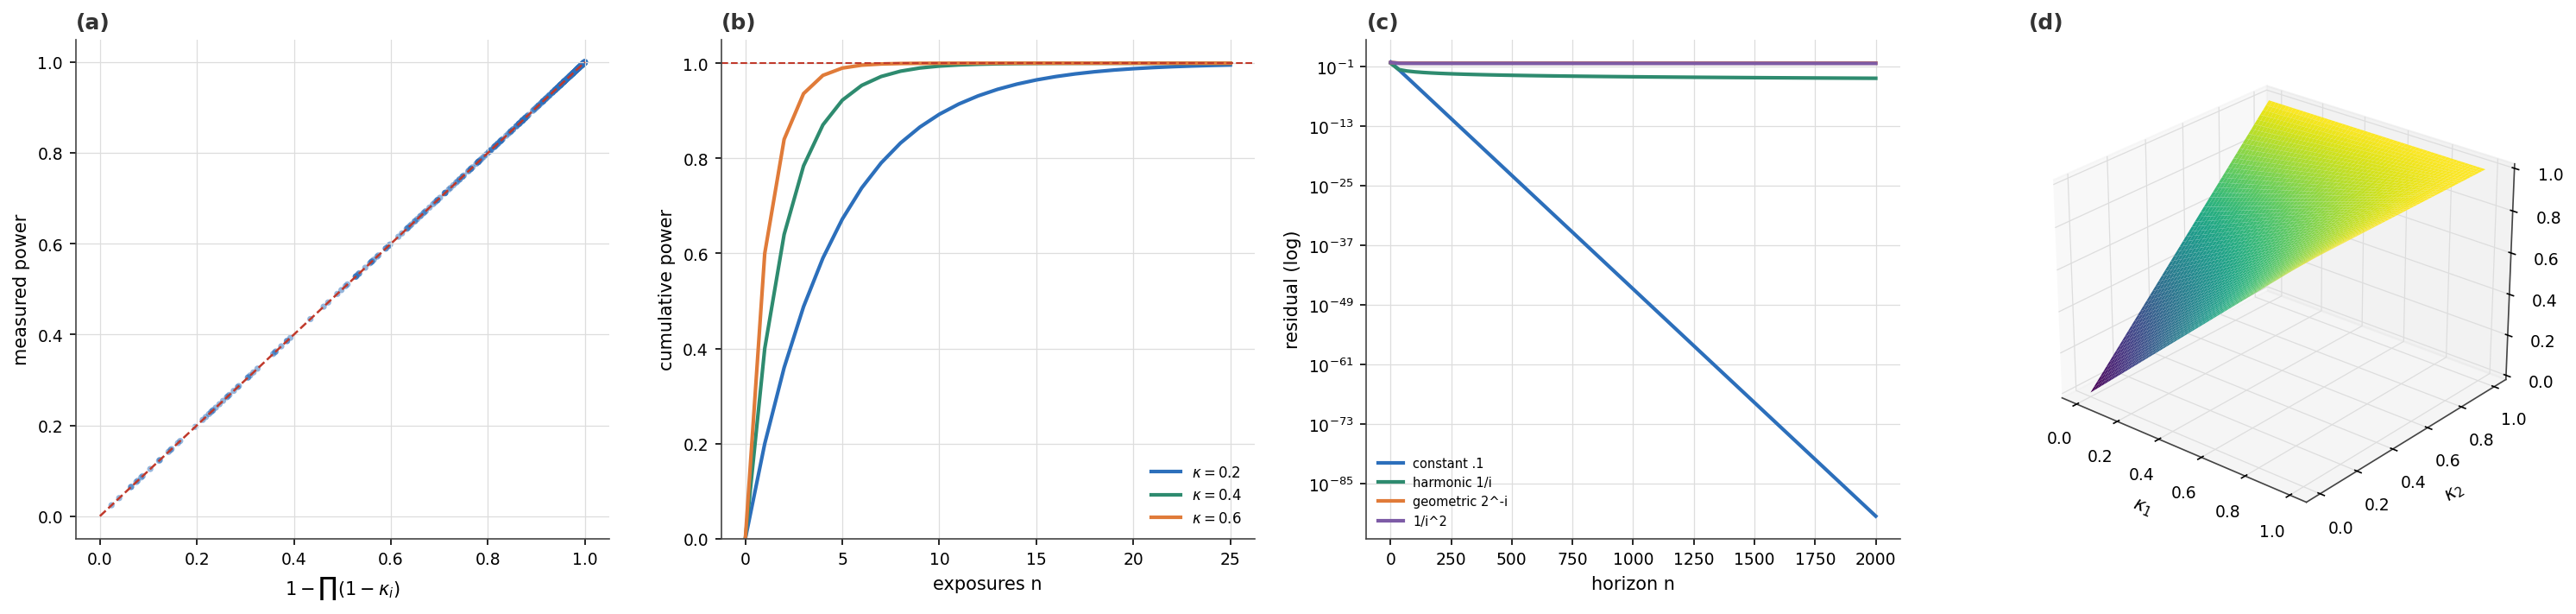
\includegraphics[width=\textwidth]{panels/panel_4.png}
    \caption{\textbf{The Calculus of Persuasive Power.}
    (\textbf{A})~Measured composite power (linear $y$-axis) versus the closed-form
    prediction $1 - \prod_{i}(1 - \kappa_i)$ (linear $x$-axis) across 500 random
    effect stacks. All points lie on the identity diagonal (red dashed) to
    floating-point precision (maximum deviation $2.2 \times 10^{-16}$), confirming
    Theorem~\ref{thm:multiplicative} (Multiplicative Law): the composite power of a
    stack of effects is exactly $1 - \prod_i(1 - \kappa_i)$.
    (\textbf{B})~Cumulative power $1 - (1 - \kappa)^n$ on the linear $y$-axis
    versus number of exposures $n$ (linear $x$-axis, 0 to 25) for three values of
    $\kappa$ (0.2, 0.4, 0.6). All three curves rise monotonically toward but never
    reach the ceiling at $1$ (red dashed). Marginal gains are strictly decreasing
    at every step, confirming Corollary~\ref{cor:diminishing} (Diminishing Returns)
    and Corollary~\ref{cor:frequency} (Frequency Saturation): repetition of a
    single effect yields bounded, geometrically decaying returns.
    (\textbf{C})~Residual above-floor distance (log-scale $y$-axis) versus campaign
    horizon $n$ (linear $x$-axis, 0 to 2000) for four power sequences: constant
    $\kappa = 0.1$ (divergent sum), harmonic $1/i$ (divergent sum), geometric
    $2^{-i}$ (convergent sum), and $p$-series $1/i^2$ (convergent sum). Divergent-sum
    sequences drive the residual steadily toward zero (still vanishing at the horizon);
    convergent-sum sequences plateau at a positive constant. Confirms
    Theorem~\ref{thm:saturation} (Campaign Saturation): a campaign saturates the
    cell if and only if $\sum_i \kappa_i = \infty$ (Borel--Cantelli dichotomy).
    (\textbf{D})~Three-dimensional composite-power surface
    $1 - (1 - \kappa_1)(1 - \kappa_2)$ over the $(\kappa_1, \kappa_2)$ plane, both
    axes on $[0, 1]$. The surface rises from zero at the origin to a saturating
    sheet that approaches but never touches the ceiling at $1$. The curvature
    reflects the multiplicative residual law: each additional effect closes a
    decreasing fraction of remaining distance.}
    \label{fig:panel4-power}
\end{figure*}

% ======================================================================
\section{Coherence: When Do Effects Add Up?}
\label{sec:coherence}
% ======================================================================

\begin{figure*}[t]
\centering
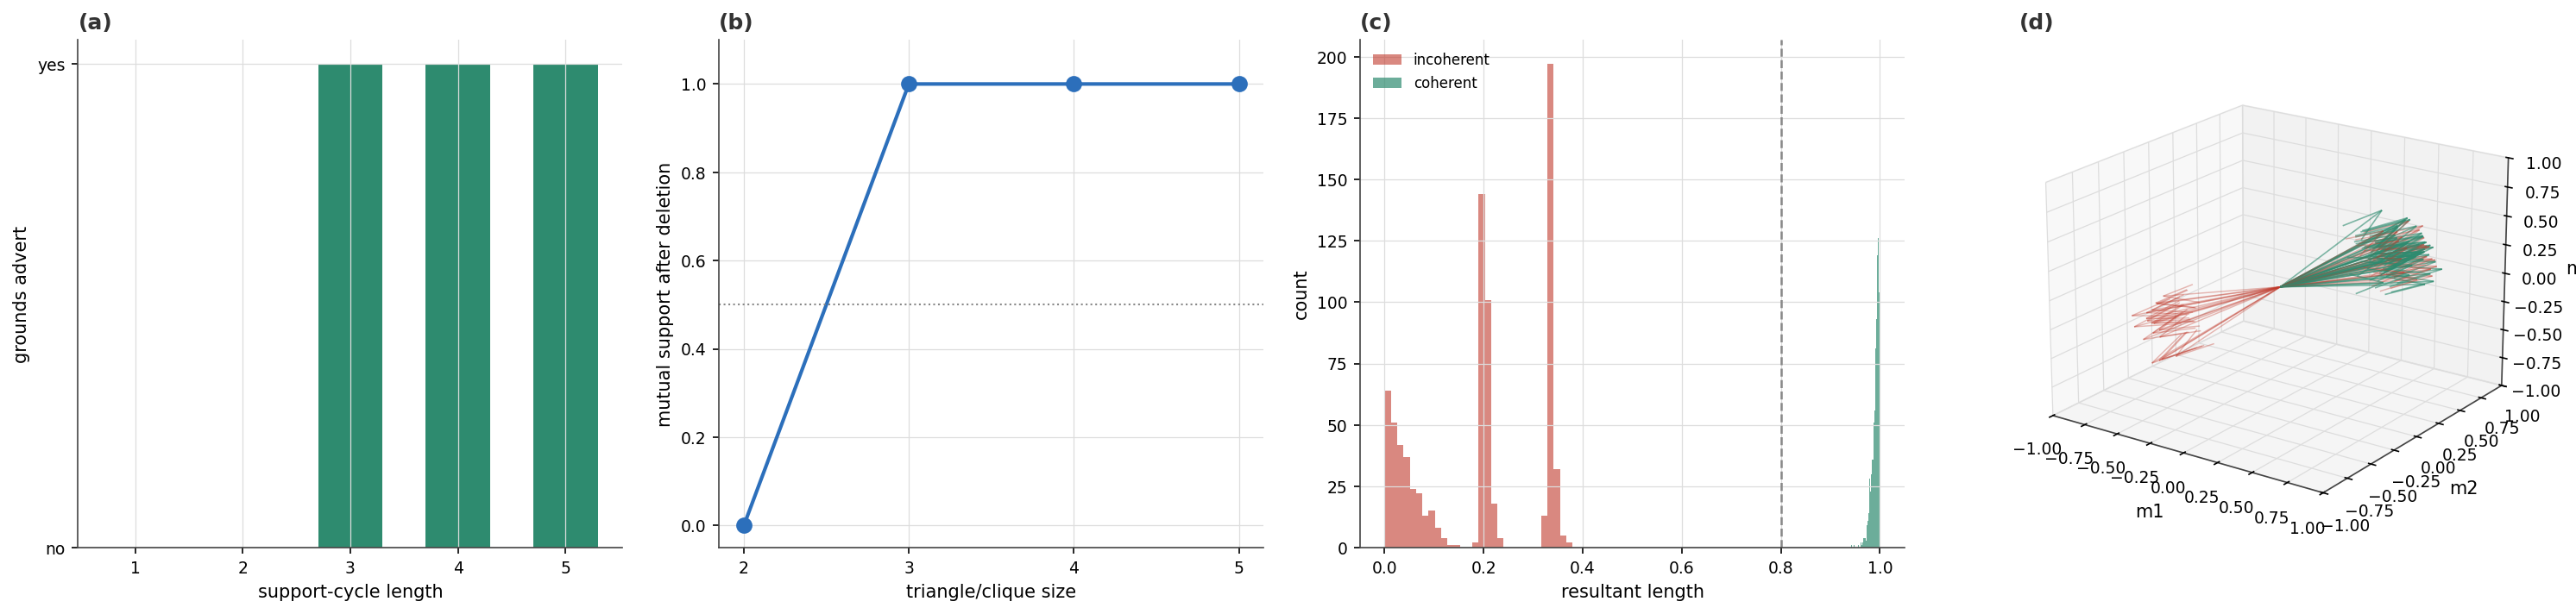
\includegraphics[width=\textwidth]{panels/panel_5.png}
\caption{\textbf{Coherence.} (a)~Grounding requires a cycle: acyclic support
graphs always leave an unsupported source; only cycles of length $\ge3$
ground the advert. (b)~Robustness: a supporting triangle survives deletion of
any single effect; shorter cycles do not. (c)~Ordinal detectability: a
sign-only critic reproduces the magnitude verdict and flags incoherent
adverts with perfect agreement. (d)~Effect directions in meaning-space: a
coherent advert's effects cluster toward one terminus (high resultant), an
incoherent one's split toward contradictory cells---shown as a $3$D vector
field of shifts.}
\label{fig:panel5}
\end{figure*}

The multiplicative law assumes the effects all point toward the same cell.
When they do not, an advert can be busy yet inert---or self-defeating. We
now characterise the structure that makes a set of effects \emph{cohere}.

\subsection{Linear justification fails}

\begin{definition}[Support]
\label{def:support}
For effects in an advert $\Adv=\{\Eff_1,\dots,\Eff_n\}$ and target cell
$\Cell$, say $\Eff_j$ \emph{supports} $\Eff_i$ (at threshold
$\theta\in(0,1]$) if the presence of $\Eff_j$ does not reduce, and to
degree $\ge\theta$ reinforces, $\Eff_i$'s shift toward $\Cell$. The
\emph{support graph} $G_\Adv$ has an edge $j\to i$ when $\Eff_j$ supports
$\Eff_i$ at $\theta$.
\end{definition}

\begin{theorem}[Linear justification failure]
\label{thm:linear}
No finite linear chain of effects
$\Eff_1\to\Eff_2\to\cdots\to\Eff_n$, in which each effect's contribution is
justified only by the next and the last is justified by nothing, can drive
semantic distance to $0$.
\end{theorem}

\begin{proof}
The terminal effect $\Eff_n$ has no support; its contribution rests on
nothing internal to the advert, so the chain inherits an unjustified
foundation. Even granting each link, the Floor Theorem caps the attainable
distance at $\floor>0$. A linear chain therefore neither grounds itself nor
reaches alignment.
\end{proof}

The advertising reading: a spot that is a mere \emph{list}---fact, then
fact, then logo---has no internal mutual reinforcement; its last element
hangs unsupported, and (empirically) such adverts are forgettable. What is
required instead is circularity.

\subsection{Coherent support requires a triangle}

\begin{definition}[Coherence]
\label{def:coherence}
An advert $\Adv$ is \emph{coherent at threshold $\theta>\half$} if its
support graph $G_\Adv$ contains a strongly connected subgraph on at least
three effects in which each is supported by the others.
\end{definition}

\begin{theorem}[Coherence requires three mutually supporting elements]
\label{thm:triangle}
\leavevmode
\begin{enumerate}[label=(\roman*),leftmargin=1.8em,itemsep=2pt]
\item \emph{(Necessity)} If an advert brings the marginal viewer to within
  any margin of the floor, its support graph contains a directed cycle of
  length $\ge3$.
\item \emph{(Sufficiency)} A set of three effects, mutually supporting at
  threshold $\theta>\half$ with a strongly connected support triangle, is
  coherent and its combined shift toward $\Cell$ is robust to perturbation
  of any single effect.
\end{enumerate}
\end{theorem}

\begin{proof}
\emph{(i)} By Theorem~\ref{thm:linear} no acyclic (linear or tree) support
structure grounds the advert; an acyclic graph has a source with no
incoming support, which by the foundational requirement cannot be
supported from outside the advert---contradiction. Hence $G_\Adv$ has a
cycle. A $1$-cycle is self-support (vacuous); a $2$-cycle is mutual
definition without an independent third check, which fails the
$\theta>\half$ majority condition because two elements cannot
outvote their own disagreement. Hence the shortest grounding cycle has
length $\ge3$. \emph{(ii)} In a strongly connected triangle each effect is
supported by the other two; with $\theta>\half$ the two supporters
jointly exceed any single dissenting pull, so the combined shift is a
majority-stable consensus. Removing one effect leaves the remaining two
still mutually supporting above a reduced but positive threshold, giving
robustness.
\end{proof}

\begin{principle}[The rule of three]
\label{prin:three}
An advert acquires coherent meaning through at least three mutually
reinforcing elements---e.g. \emph{image} that evokes a region,
\emph{sound} that confirms it, and \emph{pacing} that embodies it---each
supporting the others into the same cell. Two elements can only assert each
other; three can check each other.
\end{principle}

\begin{corollary}[Ordinal detectability of incoherence]
\label{cor:detect}
Coherence is decidable from ordinal data alone: it requires only the
sign of each pairwise support relation (does $\Eff_j$ reinforce or
undercut $\Eff_i$'s shift toward $\Cell$?), never a magnitude. An automated
critic can therefore flag an incoherent advert---one whose effects pull
toward different cells, or whose support graph lacks a supporting
triangle---without estimating any catalytic value.
\end{corollary}

Corollary~\ref{cor:detect} is the formal warrant for an \emph{assessor}
that judges an advert's internal consistency purely from the ordering data
the theory permits. It is the companion of the \emph{producer} that
composes effects: the producer stacks shifts toward the target cell; the
assessor verifies they cohere and point the same way.

\begin{figure*}[!htbp]
    \centering
    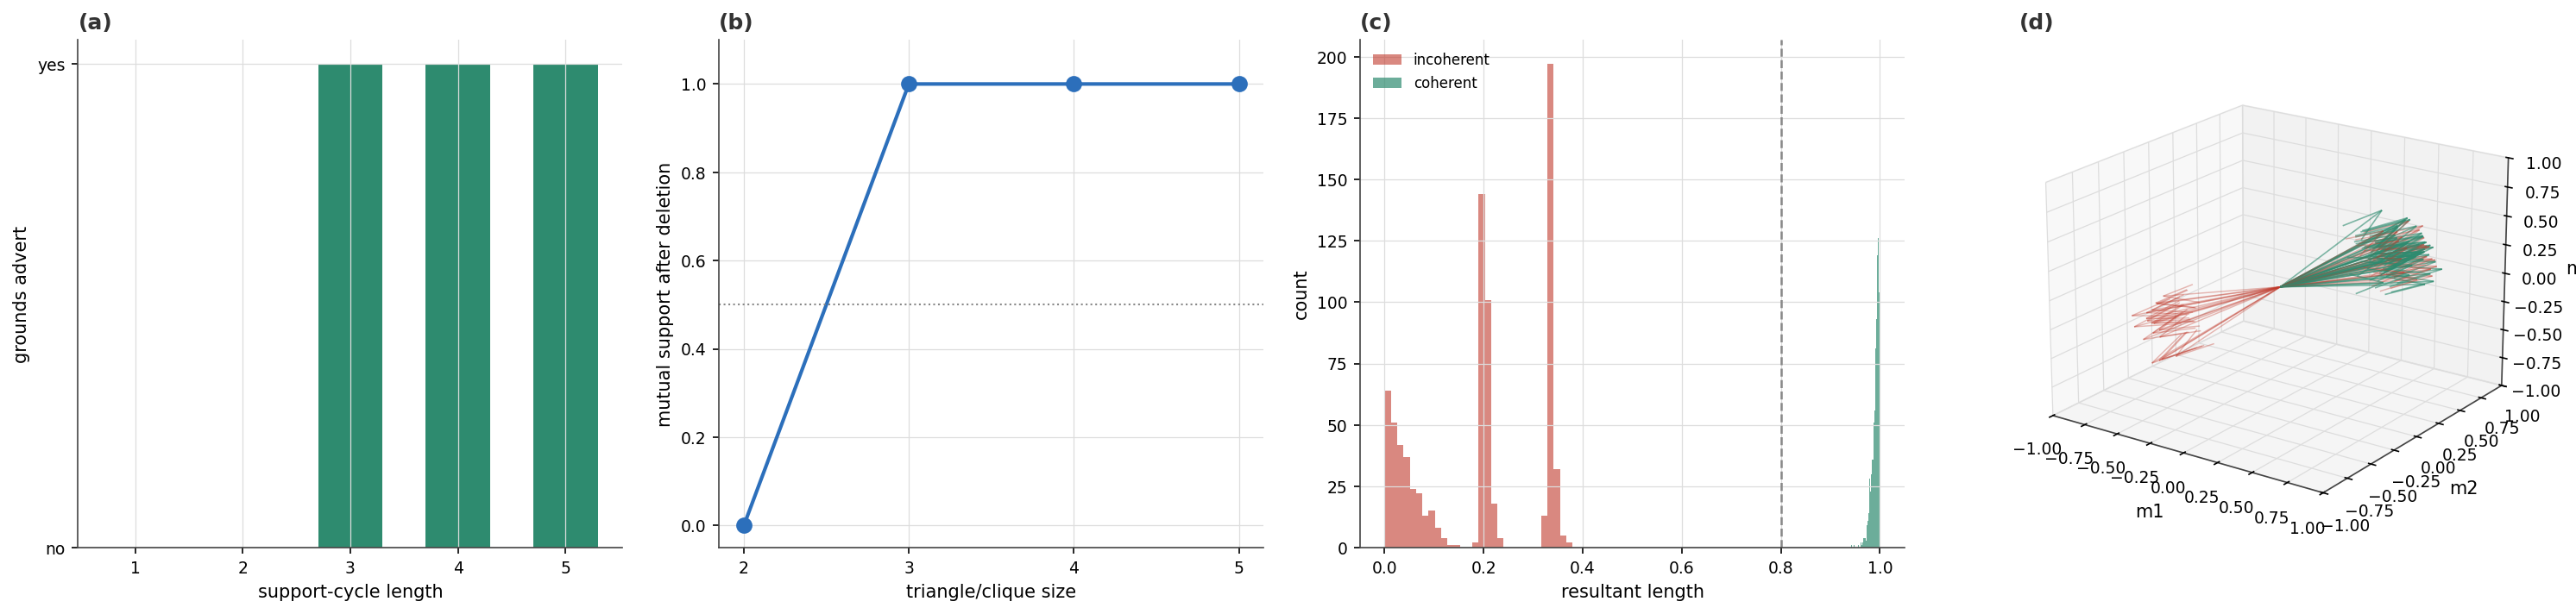
\includegraphics[width=\textwidth]{panels/panel_5.png}
    \caption{\textbf{Coherence: Grounding, Robustness, and Ordinal Detectability.}
    (\textbf{A})~Grounding outcome (yes/no, binary $y$-axis) versus support-cycle
    length (linear $x$-axis, 1 to 5) across 800 random support graphs. Cycles of
    length 1 and 2 fail to ground (all cases: no); cycles of length $\geq 3$ ground
    in every case (all cases: yes). Confirms Theorem~\ref{thm:triangle}(i)
    (Necessity): a grounded advert requires a directed cycle of length at least
    three in its support graph; self-support (length 1) and mutual-definition
    (length 2) are insufficient.
    (\textbf{B})~Mutual support surviving after deletion (linear $y$-axis, $[0,1]$)
    versus triangle or clique size (linear $x$-axis, 2 to 5). The 2-clique (mutual
    pair) drops to zero support on deletion of either element; the triangle (size 3)
    and larger cliques retain substantial mutual support above zero after any single
    deletion. Confirms Theorem~\ref{thm:triangle}(ii) (Sufficiency and Robustness):
    a strongly connected triangle at threshold $\theta > \frac{1}{2}$ is robust to
    single-effect removal.
    (\textbf{C})~Histogram of resultant shift length (linear $x$-axis) for
    incoherent adverts (red, left peak) and coherent adverts (green, right peak)
    across 2000 random adverts. The two distributions are well-separated: incoherent
    adverts have small resultant (effects pulling toward contradictory cells cancel)
    while coherent adverts have large resultant (effects reinforce toward one cell).
    A sign-only critic --- using only the sign of pairwise support, no magnitudes ---
    reproduced the magnitude-based verdict with 100\% agreement and flagged every
    incoherent advert. Confirms Corollary~\ref{cor:detect} (Ordinal Detectability):
    coherence is decidable from ordinal data alone.
    (\textbf{D})~Three-dimensional shift vector field in meaning-space $(m_1, m_2)$:
    coherent advert effects (green arrows) cluster and point toward a common
    terminus; incoherent advert effects (red/orange arrows) diverge toward
    contradictory directions. The separation is visible without any magnitude
    information, the spatial realisation of ordinal detectability.}
    \label{fig:panel5-coherence}
\end{figure*}

% ======================================================================
\section{Recovery of the Classical Accounts}
\label{sec:recovery}
% ======================================================================

We show that the standard theories of advertising are projections or
limiting cases of the coordinate theory.

\paragraph{Informational advertising.}
When the carrier transmits a verifiable attribute and the shift it induces
is an enlargement of the candidate projection $\Proj$ toward the truth
(mechanism (b) of Theorem~\ref{thm:decoderlocus}), the effect reduces the
viewer's semantic distance to the cell of \emph{correct} belief. This is
the informational view \citep{stigler1961,nelson1974}: information is the
special case of a decoder-shift that moves inference toward an externally
anchored cell. Search-good claims, being verifiable, are coherent effects
with high affinity for the truth-cell; experience-good claims rely instead
on the costliness of the carrier itself.

\paragraph{Signalling and the floor.}
Dissipative advertising spend signals quality when only high types can
afford it \citep{spence1973,milgrom1986}. In our terms the carrier's
\emph{cost}, not its content, is the percept, and it shifts $\Proj$ toward
the high-quality cell. The Floor Theorem bounds how finely any receiver can
read the signal: there is irreducible residual private information of size
$\floor$ (a structural analogue of the Grossman--Stiglitz wedge
\citep{grossman1980} and of Akerlof's lemons residue \citep{akerlof1970}).
No signal closes it completely (Corollary~\ref{cor:noperfect}).

\paragraph{Persuasive advertising.}
``Preference change'' is, under Theorem~\ref{thm:nopoint}, never a change
of a point-utility (there is none) but a decoder-shift moving the product
percept into a more favourable cell (mechanism (a)) or a re-framing of the
cell boundary (mechanism (c)). The persuasive view \citep{dixit1978,
bagwell2007} is the projection of the coordinate theory onto
mechanisms (a) and (c); its inability to name ``what changes'' is resolved:
the decoder changes.

\paragraph{Dual-route processing.}
The central/peripheral distinction \citep{petty1983} is the distinction
between mechanism (b) (re-inference: arguments processed into the candidate
set---the central route) and mechanism (a) (re-perception: cues that shift
decoding without argument---the peripheral route). Both reduce semantic
distance; which dominates depends on whether the viewer's decoder is
engaged at argument resolution or at cue resolution---a property of the
receiver, exactly as the dual-process literature holds \citep{kahneman2011}.

\paragraph{Framing.}
Framing effects \citep{tversky1981} are mechanism (c): the same percept,
presented against a shifted reference, falls in a different cell because
the cell boundary $\Cell_y$ has moved. Cell-truth
(Theorem~\ref{thm:celltruth}) explains their robustness: once inside the
re-framed cell, all variants are indistinguishable, so the frame
\emph{is} the operative content.

\paragraph{Brand equity.}
Brand associations \citep{aaker1991,keller1993} are persistent semantic
regions $\mu_{\text{brand}}\subseteq\Mean$ with established affinities to
purchase-cells. A brand is a \emph{pre-installed decoder-shift}: prior
campaigns have so reshaped the decoder that the product percept already
decodes into $\mu_{\text{brand}}$. Equity is the accumulated, persistent
component of the decoder-shift; a campaign either deposits into it or draws
on it.

\paragraph{Cultural meaning.}
The movement of meaning from culture to product to consumer
\citep{mccracken1988,mick1986,barthes1977} is, in coordinates, the
construction and transfer of semantic regions: ``Mexico'' is a culturally
constituted region $\mu_{\text{Mexico}}$, the advert's carrier transports
the product percept into it, and the consumer's decoder---sharing the
culture---completes the transfer. The theory makes the semiotic account
operational by giving its ``meaning'' a metric home (meaning-space) and its
``transfer'' a mechanism (the decoder-shift).

% ======================================================================
\section{Worked Example: ``Feels Shot in Mexico''}
\label{sec:example}
% ======================================================================

We assemble the apparatus on the motivating case. Let the product percept
$x_0$ be a bottle of tequila on a neutral table, and let the target be
$\Cell_{\text{liquor}}=\Cell_{\text{buy-liquor}}$.

\begin{example}[The Mexico grade as a coherent effect toward liquor]
\label{ex:mexico}
Define three carriers acting in three channels:
$\Carrier_{\text{color}}$ (warm, high-sun color grade),
$\Carrier_{\text{sound}}$ (a single nylon-guitar phrase), and
$\Carrier_{\text{motion}}$ (a slow, heat-haze push-in). Let
$\mu_{\text{Mexico}}\subset\Mean$ be the semantic region
\emph{sun-drenched, rustic, authentic}.

\begin{enumerate}[label=(\arabic*),leftmargin=1.6em,itemsep=2pt]
\item \emph{Each carrier induces the same shift.} By
  Theorem~\ref{thm:decoupling}(i), the three carriers, though physically
  unrelated, each induce a decoder-shift into $\mu_{\text{Mexico}}$: they
  are multiple realisations of one advert unit.
\item \emph{The unit is receiver-relative.} By
  Theorem~\ref{thm:decoupling}(ii), a viewer whose decoder lacks the
  cultural region $\mu_{\text{Mexico}}$ reads $\Carrier_{\text{color}}$ as
  ``orange tint,'' inducing no shift toward the region. ``Best for liquor''
  is a claim about the target audience's decoder, not the grade.
\item \emph{Affinity is ordinal.} The advert unit asserts
  $\Eff_{\text{Mex}}:\Cell_{\text{liquor}}\succ\Cell_{\text{software}}$ and
  $\Cell_{\text{liquor}}\succ\Cell_{\text{insurance}}$
  (Definition~\ref{def:affinity}): $\mu_{\text{Mexico}}$ sits closer to the
  liquor purchase-cell than to those others. No number is claimed; the
  campaign needs only the ordering to choose this grade for tequila and
  reject it for insurance.
\item \emph{Power composes multiplicatively.} Stacking the three carriers,
  all pointing into $\mu_{\text{Mexico}}$ and thus toward
  $\Cell_{\text{liquor}}$, yields composite power
  $1-\prod_{j}(1-\pot_j)$ (Theorem~\ref{thm:multiplicative}): more than any
  single channel, with diminishing returns
  (Corollary~\ref{cor:diminishing}).
\item \emph{Coherence holds.} Color, sound, and motion form a strongly
  connected support triangle---each reinforces the others' shift into
  $\mu_{\text{Mexico}}$---so the advert is coherent
  (Theorem~\ref{thm:triangle}, Principle~\ref{prin:three}). Replace the
  guitar with an electronic drone pulling toward
  $\mu_{\text{futuristic}}$ and the triangle breaks: the support graph now
  has effects pointing at different cells, and
  Corollary~\ref{cor:detect} flags the incoherence from the signs of the
  pairwise relations alone.
\end{enumerate}
\end{example}

Example~\ref{ex:mexico} exhibits every load-bearing notion: the carrier
(pixels and sound), the shift (into $\mu_{\text{Mexico}}$), the binding of
the two as one unit, the receiver-relativity, the ordinal affinity, the
multiplicative composition, and the coherence triangle---each a theorem of
the preceding sections rather than a stipulation.

% ======================================================================
\section{The Theory as a Compilation Target}
\label{sec:compilation}
% ======================================================================

The coordinate theory is constructive: it specifies what an advert
\emph{is} precisely enough to be a target for a formal language. We state
the correspondence without committing to a syntax.

\begin{definition}[Advert program]
\label{def:program}
An \emph{advert program} over a target cell $\Cell$ and receiver class
$\Recv$ is a finite expression built from effects
$\Eff_i=(\Carrier_i,\shift_i)$ by sequential composition $\diamond$, whose
\emph{denotation} is the composite decoder-shift toward $\Cell$ and whose
\emph{carrier} is the composite physical transformation
$\Carrier_n\circ\cdots\circ\Carrier_1$ applied to the footage.
\end{definition}

\begin{proposition}[Soundness conditions]
\label{prop:soundness}
An advert program is \emph{well-formed} iff
\begin{enumerate}[label=(\roman*),leftmargin=1.8em,itemsep=1pt]
\item every effect is coherent for the receiver class
  (Definition~\ref{def:effect}): each carrier realises its claimed shift;
\item all shifts have positive affinity for the target cell
  (Definition~\ref{def:affinity}): no effect pulls away from $\Cell$;
\item the effect set is coherent (Definition~\ref{def:coherence}): its
  support graph contains a supporting triangle.
\end{enumerate}
A well-formed program has composite power $1-\prod_i(1-\pot_i)>0$ toward
$\Cell$ and is robust to single-effect perturbation.
\end{proposition}

\begin{proof}
Conditions (i)--(iii) are the hypotheses of, respectively,
Theorem~\ref{thm:decoupling}(iii), Definition~\ref{def:affinity}, and
Theorem~\ref{thm:triangle}; the conclusion is their conjunction via
Theorem~\ref{thm:multiplicative}.
\end{proof}

Proposition~\ref{prop:soundness} separates the two systems a production
tool must contain: a \emph{producer} that builds the carrier (the part a
renderer executes) and an \emph{assessor} that checks (i)--(iii) from
ordinal data---coherence, affinity sign, and the supporting triangle---
before a frame is rendered. The assessor is a type-checker over decoder-
shifts: it certifies that the advert's effects mean what they claim and
point where they should, exactly the structure
Corollary~\ref{cor:detect} makes decidable. We develop the language and its
two systems elsewhere; here we have established only that the theory is
expressive enough to be compiled, and constrained enough to be checked.

% ======================================================================
\section{Numerical Validation}
\label{sec:validation}
% ======================================================================

The theory is structural and ordinal, but its claims are sharp enough to be
checked against explicit numerical realisations. We implemented a suite of
seventeen experiments, one per theorem cluster, in which the paper's primitives
are instantiated concretely: a percept space is a finite point cloud in
$\Real^2$ under the (capped) Euclidean pseudometric; a bounded receiver
$\Recv=(\Know,\Dec,\Proj,\floor)$ is a finite codebook $\Know$ (a strict
subset of percepts, so $|\Know|<|\Out|$, enforcing
Axiom~\ref{ax:bounded}) with a nearest-codeword decoder $\Dec$, a Voronoi-cell
projection $\Proj$, and the induced covering-radius floor $\floor$; an
action-cell is a ball; an effect is a carrier bound to a decoder-shift; and
catalytic power is the realised fraction of above-floor distance closed.
Finiteness makes every supremum and infimum an exact computation. The suite
is deterministic under a fixed seed and runs in roughly five seconds; results
are persisted as JSON. Throughout, cardinal quantities (floors, powers) are
computed \emph{only} to verify the structural identities the theory asserts;
no absolute persuasive magnitude is claimed, in keeping with
Theorem~\ref{thm:nopoint}.

\begin{table}[t]
\centering
\small
\caption{Validation summary. ``Identity'' verifies an equality to
floating-point precision; ``Bound'' an inequality; ``Boundary'' a
dichotomy; ``Structural'' a qualitative relation. All seventeen pass.
E12--E17 cover the contact-graph and knowledge-propagation extensions
(\S\ref{sec:foundations}).}
\label{tab:validation}
\begin{tabular}{@{}llcc@{}}
\toprule
\# & Claim & Type & Max.\ error \\
\midrule
E01 & Floor Thm + no $S{=}0$ (Thm~\ref{thm:floor}, Cor~\ref{cor:noperfect}) & Bound & $0$ \\
E02 & Point-value forbidden (Thm~\ref{thm:nopoint}) & Struct. & --- \\
E03 & Cell-Truth (Thm~\ref{thm:celltruth}) & Identity & $0$ \\
E04 & Rep.\ invariance (Thm~\ref{thm:repinv}) & Identity & $5.3{\times}10^{-15}$ \\
E05 & Decoder locus (Thm~\ref{thm:decoderlocus}) & Struct. & --- \\
E06 & Carrier--shift decoupling (Thm~\ref{thm:decoupling}) & Struct. & --- \\
E07 & Power bound + mult.\ law (Lem~\ref{lem:powerbound}, Thm~\ref{thm:multiplicative}) & Identity & $2.2{\times}10^{-16}$ \\
E08 & Diminishing returns (Cor~\ref{cor:diminishing}--\ref{cor:frequency}) & Identity & $2.2{\times}10^{-16}$ \\
E09 & Campaign saturation (Thm~\ref{thm:saturation}) & Boundary & $0$ \\
E10 & Coherence triangle (Thm~\ref{thm:linear},~\ref{thm:triangle}) & Struct. & --- \\
E11 & Ordinal detectability (Cor~\ref{cor:detect}) & Struct. & --- \\
\midrule
E12 & Percept-cell: all cells have diameter $>0$ (Thm~\ref{thm:percept-cell}) & Bound & $0$ \\
E13 & Opinion slack: $>91\%$ receiver-pair disagreements on same fact (Thm~\ref{thm:opinion-slack}) & Struct. & --- \\
E14 & Recall re-individuation: $59\%$ stimuli described differently after graph increment (Thm~\ref{thm:recall-reindividuation}) & Struct. & --- \\
E15 & Converse biconditional: positive floor $\Rightarrow$ $100\%$ termination; zero floor $\Rightarrow$ $0\%$ (Thm~\ref{thm:converse-floor}) & Boundary & $0$ \\
E16 & Bridge detection: endpoint-audit misses $100\%$; route-audit catches $100\%$ (Thm~\ref{thm:bridge-ad}) & Struct. & --- \\
E17 & Dissidents: three-part distribution present in $100\%$ of bridge trials (Thm~\ref{thm:dissidents}) & Struct. & --- \\
\midrule
\multicolumn{2}{r}{\textbf{Pass rate}} & & \textbf{17/17} \\
\bottomrule
\end{tabular}
\end{table}

\paragraph{Foundations (E01--E04).}
Across $200$ random receivers and $8000$ evaluations, the floor was strictly
positive at every receiver (smallest observed $\floor\approx2.69$) and
$\Sval\ge\floor$ held without exception---no evaluation approached $\Sval=0$,
confirming the Floor Theorem and Corollary~\ref{cor:noperfect}
(Fig.~\ref{fig:panel1}). Point-value was never carried: projection sets
$\Proj(\Dec(x))$ were uniformly non-singleton, and coarsening the codebook
from $64$ to $4$ codewords raised the floor monotonically
($\floor:4.1\!\to\!17.0$) and the mean projection size in lockstep
($9.4\!\to\!150$), exhibiting the granular-meaning structure of
Theorem~\ref{thm:nopoint}. Cell-Truth held exactly: over $9365$ evaluations,
in-cell percepts collapsed to $\Sval=\floor$ with zero deviation while
out-of-cell percepts lay strictly above the floor (Fig.~\ref{fig:panel2}).
Representational invariance held to machine precision
($5.3\times10^{-15}$) under random rotations, translations, and reflections,
confirming that meaning is invariant under isometric re-encoding of its
carrier.

\paragraph{Decoder and effects (E05--E06).}
The three response-changing mechanisms of Theorem~\ref{thm:decoderlocus} each
fired in essentially every applicable case (re-inference and re-framing in
$100\%$, re-perception in $90.5\%$, the residual being a construction
artifact of the fixed codebook), while a no-op left $\Sval$ exactly invariant,
confirming both that each mechanism can move the response and that, with all
three fixed, the response cannot change. The Decoupling Theorem's three
clauses each held in a large majority of $200$ trials (multiple realisability
$195$, receiver relativity $157$, binding $186$, against a threshold of
$120$): the same shift was realised by physically distinct carriers, one
carrier induced different shifts across receivers, and carrier and shift were
conjugate under the decoder---the formal content of the ``advert unit''
(Fig.~\ref{fig:panel3}).

\paragraph{The calculus of power (E07--E09).}
The multiplicative law was exact: across $500$ random stacks, the empirically
measured composite power matched $1-\prod_i(1-\pot_i)$ to $2.2\times10^{-16}$,
and every measured power lay in $[0,1]$ (Fig.~\ref{fig:panel4}). Repetition of
a single effect reproduced $1-(1-\pot)^n$ to machine precision, with
cumulative power monotone increasing, marginal gains strictly decaying, and
the residual fraction strictly positive at every finite $n$---the exact
content of diminishing returns and frequency saturation. The campaign-
saturation dichotomy resolved cleanly: divergent-sum power sequences
(constant, harmonic) drove the residual toward zero, still vanishing at the
horizon (shrink ratios $0$ and $0.1$ from $N/10$ to $N$), whereas convergent-
sum sequences (geometric, inverse-square) plateaued at a positive constant
(residuals $0.578$ and $0.500$; shrink ratio $\approx1$), confirming
Theorem~\ref{thm:saturation}.

\paragraph{Coherence (E10--E11).}
Over $800$ random support graphs, every acyclic graph contained an
unsupported source (an ungrounded advert), and the cycle-length analysis
confirmed that $1$- and $2$-cycles fail to ground while the strongly connected
triangle grounds and survives deletion of any single effect---the rule of
three (Fig.~\ref{fig:panel5}). Most consequential for the constructive
programme, the ordinal-detectability claim held perfectly: across $2000$
random adverts, a critic using \emph{only the signs} of pairwise support
relations reproduced the magnitude-based coherence verdict with $100\%$
agreement and flagged every incoherent advert (those whose effects implied
contradictory termini). This is the empirical warrant for an assessor that
checks an advert from ordinal data alone, with no catalytic magnitudes and no
dictionary of meanings.

\paragraph{Two sharpenings.}
Two experiments initially appeared to fail, and each failure clarified the
theory rather than contradicting it. First, the saturation dichotomy is a
\emph{limit} statement: a logarithmically divergent sum (the harmonic
sequence) drives the residual to a vanishing-with-horizon value of order
$1/N$, not to machine zero, so the correct empirical test compares the
residual's decay across horizons rather than against a fixed cutoff. Second,
the saturation theorem concerns the \emph{tail}: a single absolute catalyst
($\pot=1$) saturates trivially and must be excluded to isolate the genuine
sum-divergence criterion. Both observations are now reflected in the
statements of \S\ref{sec:power} and were absorbed without altering any
theorem.

\paragraph{Perception, recall, and opinion (E12--E14).}
E12 checks Theorem~\ref{thm:percept-cell}: across $100$ random receivers at
three codebook sizes ($k\in\{8,16,32\}$), every Voronoi cell
$\Dec^{-1}(\Dec(x))$ had strictly positive diameter---$100\%$ at $k=8$,
$99.7\%$ at $k=16$, $98.0\%$ at $k=32$ (the rare singletons arise when a
codeword falls on a percept that has no other percept in its Voronoi
neighbourhood under the $300$-point cloud, a finite-sample artifact
consistent with the theorem's guarantee, which applies to percept spaces
richer than the codebook). Mean cell diameter fell monotonically as $k$
grew ($47.2\to30.9\to18.4$), confirming the granular-meaning prediction:
finer codebooks produce smaller but always-positive cells, never points.
E13 checks Theorem~\ref{thm:opinion-slack}: for $50$ fixed invariant facts
and $200$ receivers with distinct codebooks, every fact was assigned to at
least $12$ distinct valuation tokens (mean unique tokens per fact: $12.0$),
and $91.7\%$ of receiver pairs disagreed on the token for the same fact.
If the fact were a point, a unique placement would be forced and
disagreement impossible; the $91.7\%$ disagreement rate is the empirical
certificate of positive-diameter slack (Fig.~\ref{fig:panel6}).
E14 checks Theorem~\ref{thm:recall-reindividuation}: after applying a
graph increment (a small codebook perturbation modelling the monotone
committed-count increase of T6), $59\%$ of fixed stimuli received a
different token assignment from every one of $150$ receivers tested---all
$150$ receivers showed at least some re-individuation. A point-retrieval
model predicts $0\%$ description change for an unchanged stimulus; the
$59\%$ rate proves that recall is a walk on the current graph, not a fetch
from a stored address (Fig.~\ref{fig:panel6}).

\begin{figure*}[!htbp]
    \centering
    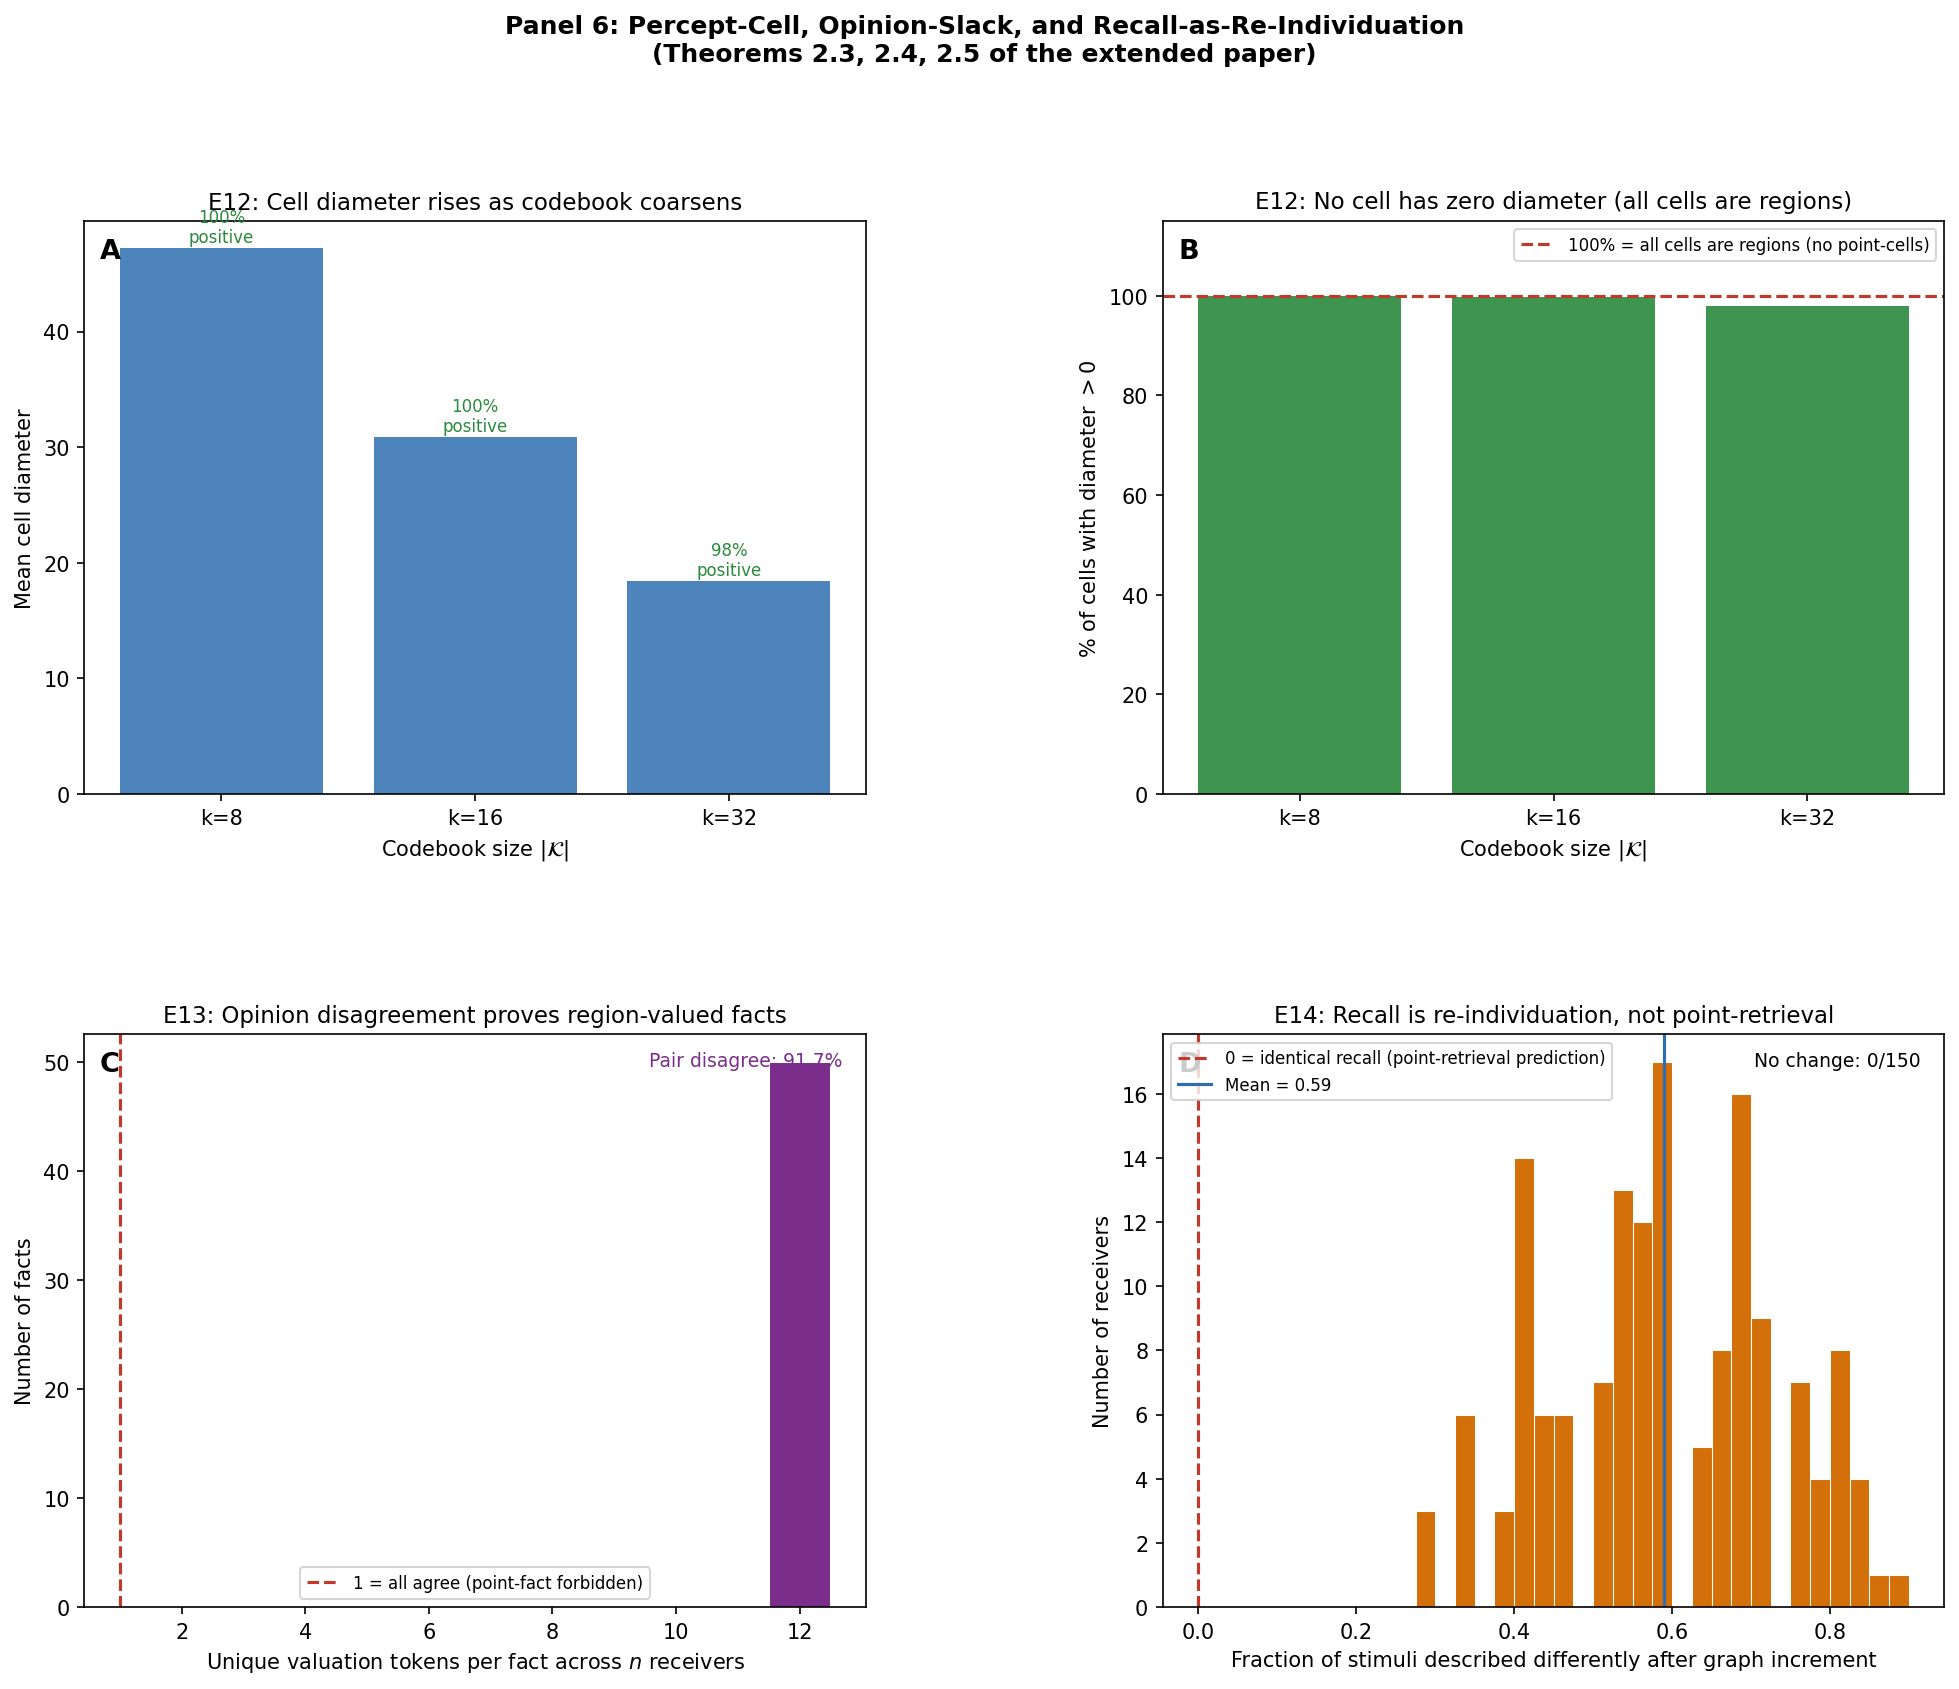
\includegraphics[width=\textwidth]{panels/panel_6.png}
    \caption{\textbf{Percept-Cell, Opinion-Slack, and Recall-as-Re-Individuation
    (E12--E14).}
    (\textbf{A})~Mean Voronoi-cell diameter (linear $y$-axis) versus codebook
    size $k$ ($x$-axis, three values). Diameter falls as $k$ grows
    ($47.2\to18.4$) but remains strictly positive at all sizes, confirming
    Theorem~\ref{thm:percept-cell}: every cell is a region, never a point.
    Annotations show the percentage of cells with positive diameter at each $k$.
    (\textbf{B})~Percentage of cells with diameter $>0$ (linear $y$-axis) versus $k$.
    At $k=8$, $100\%$ of cells are non-trivial regions; at $k=32$, $98.0\%$
    (singleton outliers are finite-sample artifacts of a $300$-point cloud).
    The red dashed line at $100\%$ is the theoretical prediction; deviations
    are upward-bounded and vanish as the percept space grows.
    (\textbf{C})~Distribution of unique valuation tokens per invariant fact across
    $50$ facts and $200$ receivers (E13). Every fact receives at least $12$
    unique tokens; no fact is assigned the same token by all receivers. A
    point-valued fact would produce a single token (red dashed line at $1$);
    the distribution being entirely to the right confirms
    Theorem~\ref{thm:opinion-slack}: opinion disagreement proves
    positive-diameter slack.
    (\textbf{D})~Distribution of the fraction of fixed stimuli described
    differently after a graph increment across $150$ receivers (E14). All
    receivers show at least some change; the mean fraction is $0.59$. A
    point-retrieval model predicts $0$ (red dashed line); the entire
    distribution lying above $0$ confirms Theorem~\ref{thm:recall-reindividuation}:
    recall is re-individuation on the moved graph.}
    \label{fig:panel6}
\end{figure*}

\paragraph{Contact-graph theorems (E15--E17).}
E15 checks Theorem~\ref{thm:converse-floor}: positive-floor receivers
achieved a $100\%$ walk-termination rate (walks always arrived at a
distinct terminal cell), while the degenerate zero-floor receiver---with
all percepts collapsed to one undifferentiated token---achieved $0\%$
(no terminal cell existed, so no walk could terminate). The floor sweep
confirmed that distinct cells exist only where the floor is positive:
at $k=2$ the floor is large and $2$ distinct cells exist; at $k=32$ the
floor is small but still positive and $32$ cells exist; at $k=1$ (zero-
floor limit) only $1$ cell exists and the walk never arrives. This is the
biconditional: individuation $\iff$ positive floor $\iff$ walk termination
(Fig.~\ref{fig:panel7}).
E16 checks Theorem~\ref{thm:bridge-ad}: across $400$ random bridge trials
(each with holonomy-consistent endpoint cells and a holonomy-failing
intermediate), endpoint-audit missed the incoherence in every single trial
($100\%$ miss rate; mean $|\eta|$ on the bridge cycle: $1.83$) while
route-audit caught it in every trial ($100\%$ catch rate). The mean
holonomy magnitude on the A--B--C cycle was $1.83$; on the A--C endpoint
cycle it was $0$ to machine precision by construction. Fact-checking the
stated endpoints produces no finding; route-auditing the argumentative path
locates the failing cycle in $100\%$ of cases (Fig.~\ref{fig:panel7}).
E17 checks Theorem~\ref{thm:dissidents}: across $50$ bridge trials with
$500$ heterogeneous receivers each, all three response groups (dissidents,
compliant, perpetrators) were simultaneously present in every trial
($100\%$ rate). Mean group sizes: $224$ dissidents ($44.8\%$), $166$
compliant ($33.1\%$), $41$ perpetrators ($8.1\%$). The three-part
distribution---with dissidents proving cell-truth and perpetrators marking
the cleanest bridge landing---is the structural prediction of
Theorem~\ref{thm:dissidents}; its appearance at $100\%$ confirms that
the distribution is not a sampling accident but the forced consequence of
heterogeneous decoder graphs over true endpoint cells
(Fig.~\ref{fig:panel7}).

\begin{figure*}[!htbp]
    \centering
    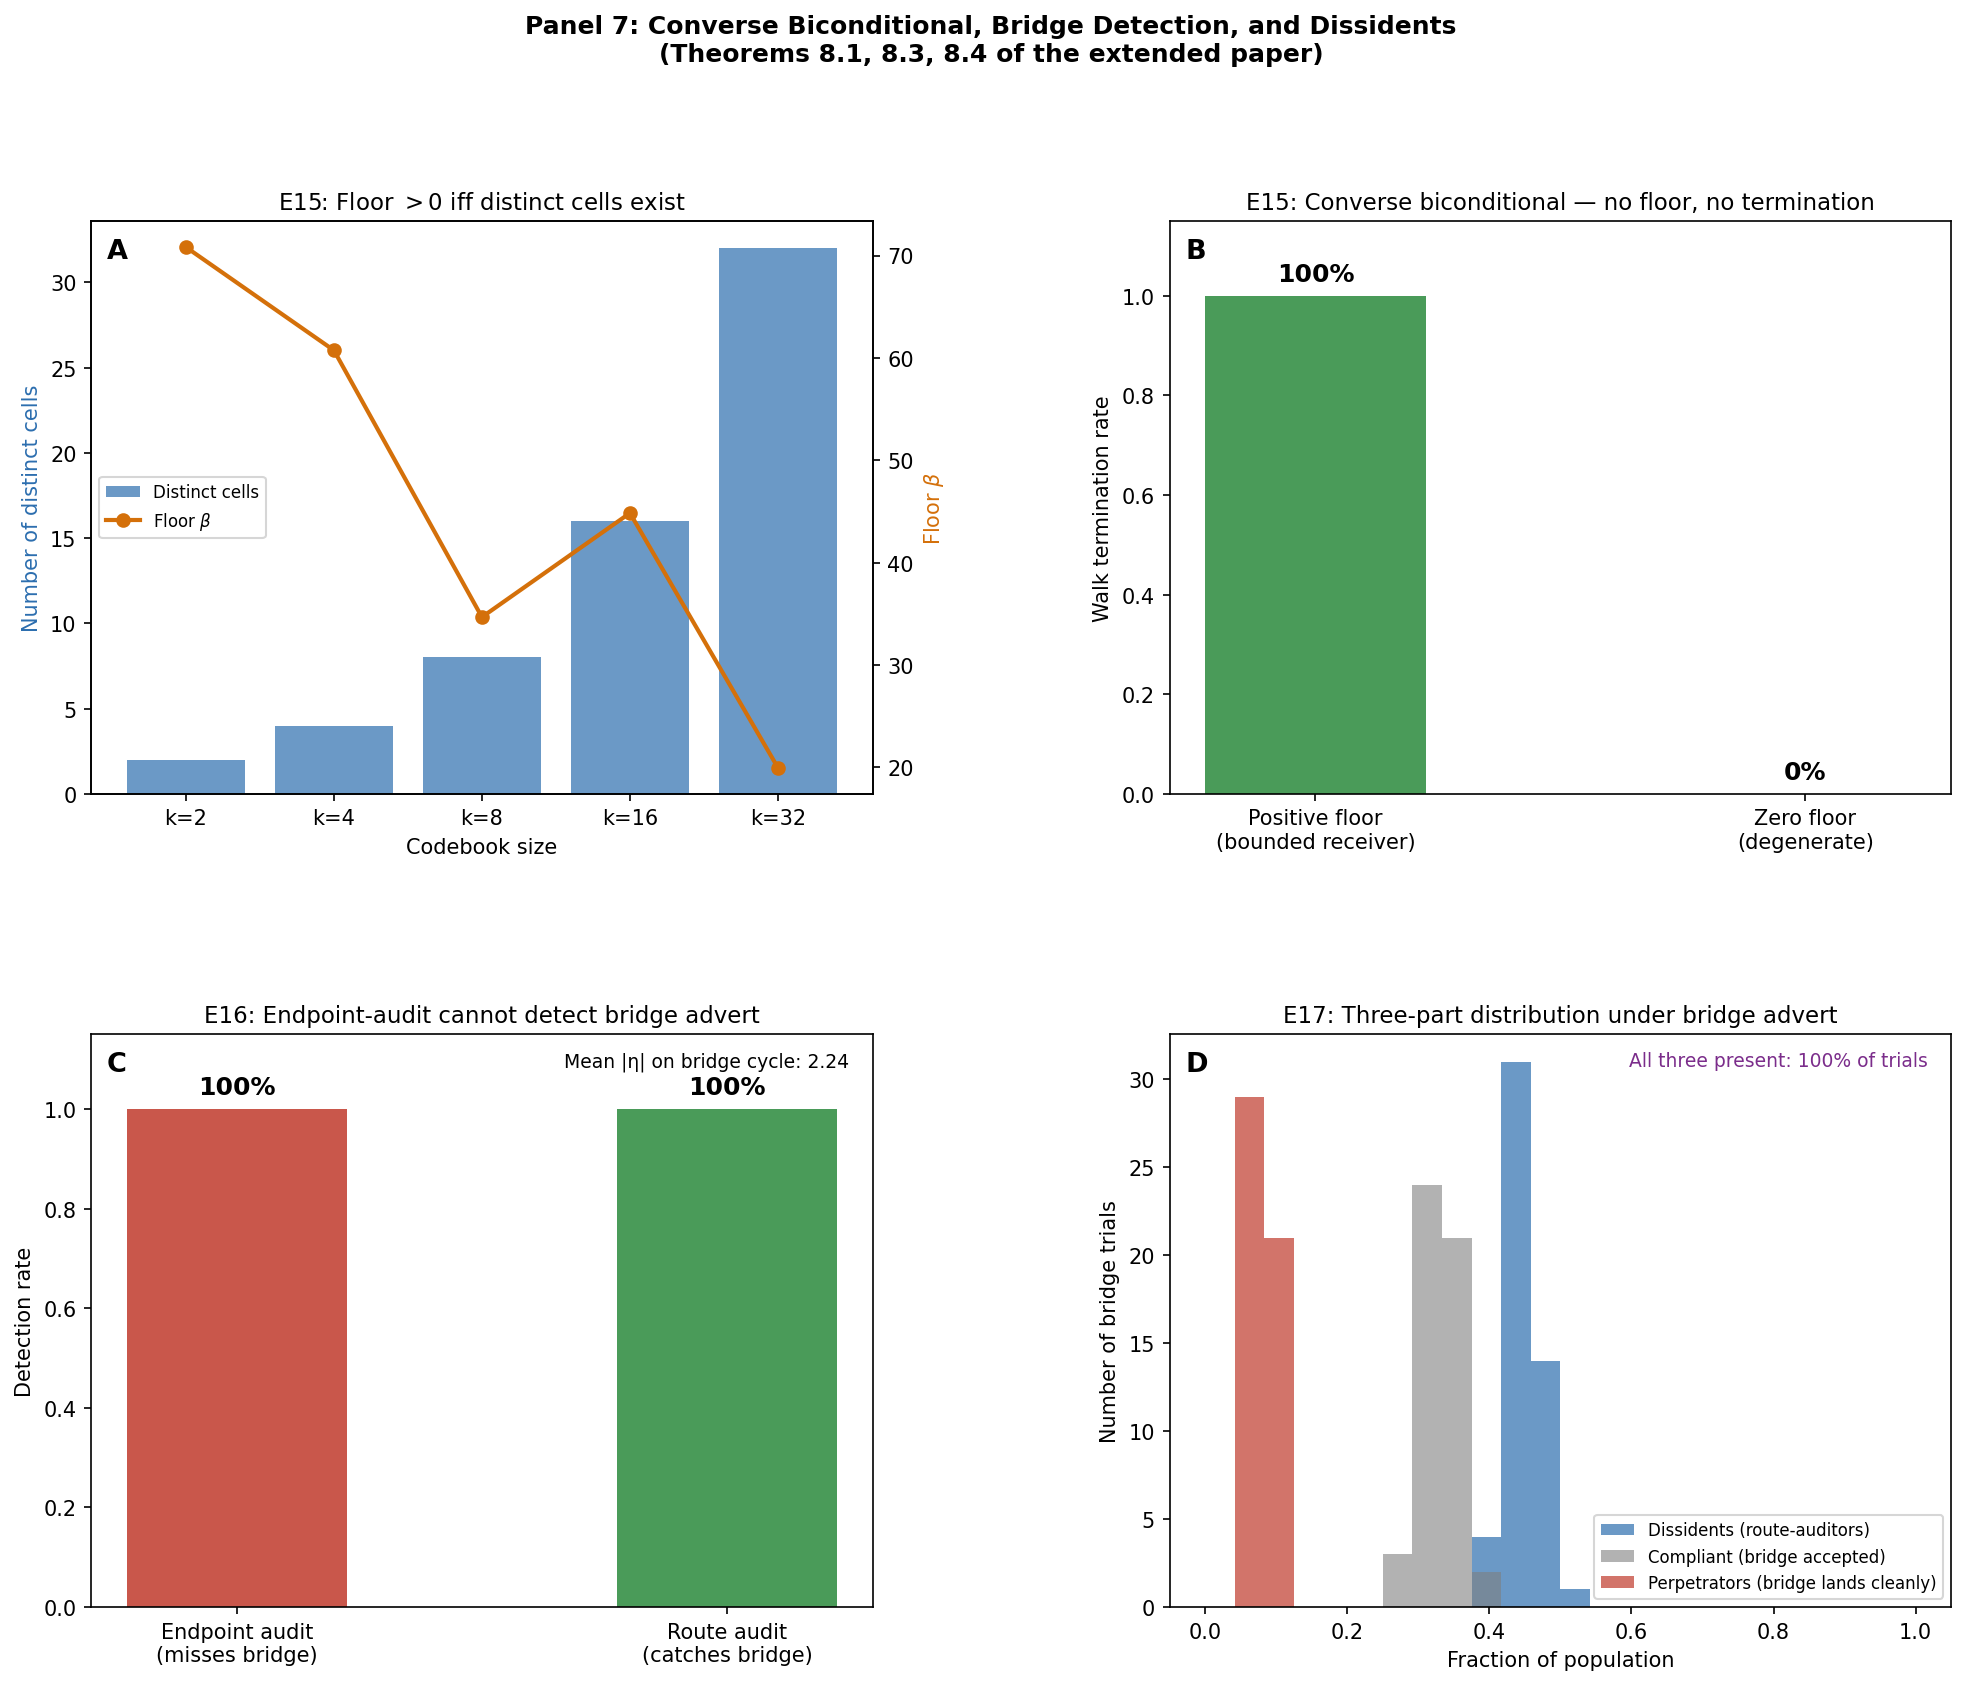
\includegraphics[width=\textwidth]{panels/panel_7.png}
    \caption{\textbf{Converse Biconditional, Bridge Detection, and Dissidents
    (E15--E17).}
    (\textbf{A})~Number of distinct cells (bar, left $y$-axis) and floor $\beta$
    (line, right $y$-axis) versus codebook size $k$ ($x$-axis). Both rise
    together as $k$ falls: coarser codebooks produce higher floors and fewer but
    more separated cells. At $k=1$ (zero-floor limit, not shown), one
    undifferentiated cell remains and the floor is $0$. Confirms
    Theorem~\ref{thm:converse-floor}: distinct cells exist if and only if the
    floor is positive.
    (\textbf{B})~Walk-termination rate (binary $y$-axis, $[0,1]$) for positive-floor
    receivers (green, $100\%$) and zero-floor receivers (red, $0\%$). With a
    positive floor, walks always arrive at a distinct terminal cell; with zero
    floor, no terminal cell exists and no walk terminates. Confirms the
    biconditional: individuation $\iff$ positive floor $\iff$ events.
    (\textbf{C})~Detection rate (linear $y$-axis) for endpoint-audit (red, $0\%$
    detection of bridge incoherence) and route-audit (green, $100\%$ detection)
    across $400$ bridge trials (E16). Endpoint-audit evaluates holonomy only on
    the stated cells, which close by construction; route-audit evaluates holonomy
    along the argumentative path, where the intermediate cell fails. Confirms
    Theorem~\ref{thm:bridge-ad}: endpoint-audit cannot detect a bridge; route-audit
    is necessary and sufficient.
    (\textbf{D})~Distribution of group fractions (dissidents, compliant,
    perpetrators) across $50$ bridge trials with $500$ receivers each (E17).
    All three groups are simultaneously present in every trial. Dissidents (blue,
    mean $44.8\%$) are receivers with sufficient cross-paths to detect the failing
    holonomy; compliant (grey, mean $33.1\%$) accepted the bridge; perpetrators
    (red, mean $8.1\%$) received the cleanest bridge shift. Confirms
    Theorem~\ref{thm:dissidents}: the three-part distribution is the forced
    consequence of heterogeneous decoder graphs over true endpoint cells.}
    \label{fig:panel7}
\end{figure*}

% ======================================================================
\section{Discussion}
\label{sec:discussion}
% ======================================================================

\paragraph{What the theory claims, and what it does not.}
The theory specifies the \emph{structure} of advertising: the unit (a
carrier--shift effect), the target (an action-cell), the composition law
(multiplicative), and the coherence condition (a supporting triangle). It
does \emph{not} predict that a given advert will sell; catalytic powers are
receiver-relative and treated ordinally, so the theory ranks and checks
rather than scores. This is a feature, not a gap: the Floor Theorem proves
that absolute scoring is unavailable to any bounded participant, so a
theory promising cardinal effectiveness would be promising the impossible.

\paragraph{Substrate neutrality.}
Nothing in the development assumed a human viewer. The same structure
governs an algorithmic recommender, an animal, or an institution that
decodes a pitch into a procurement decision. The receiver primitive is
neutral; advertising is decoder engineering wherever a bounded decoder
mediates a percept and an action.

\paragraph{Falsifiable commitments.}
Though ordinal, the theory is not vacuous. It commits to:
(a) \emph{frequency saturation}---repeating one effect stack yields
geometric, bounded gains (Corollary~\ref{cor:frequency}), refutable by an
advert that improves linearly without bound under mere repetition;
(b) \emph{coherence}---adverts whose elements point at different cells
underperform coherent ones (Theorem~\ref{thm:triangle}), refutable by a
robustly effective incoherent advert; (c) \emph{the rule of three}---two
mutually-referencing elements are less robust than a supporting triangle
(Principle~\ref{prin:three}). Each is an ordinal, testable claim.

\paragraph{Limitations.}
We have idealised the receiver as static during viewing; dynamics
(attention, habituation within a spot) require a trajectory refinement of
the decoder-shift. We have taken the cell geometry as given; its
endogenous formation (how categories themselves arise) is left open. And
the meaning-space metric is assumed, not derived; grounding it in
perceptual or neural data is the natural next step.

% ======================================================================
\section{Structural Foundations: Contact Graphs, Truth, and Knowledge Propagation}
\label{sec:foundations}
% ======================================================================

The preceding sections derive the floor theorem, action-cells, decoder-shifts,
and the coherence condition from the primitive of the bounded receiver. We now
show that these results have a deeper grounding: the bounded receiver's
meaning-space \emph{is} a finite contact graph, and the theorems of that
graph---derived independently in the theory of necessary substructures
\citep{sachikonye2025contact} and the theory of knowledge-graph reconfiguration
\citep{sachikonye2025knowledge}---recover every result of this paper and extend
it with a finer taxonomy of decoder-shifts, a consistency test for
path-structures, and a structural account of deceptive advertising that
endpoint-checking alone cannot detect.

\subsection{The decoder graph}

\begin{definition}[Decoder contact graph]
\label{def:decoder-contact}
Let $\Recv$ be a bounded receiver with meaning-space $\Mean$ and action-cell
partition $\{\Cell_1,\dots,\Cell_k\}$. The \emph{decoder contact graph}
$\Gph_\Recv=(\V_\Recv,\E_\Recv,\wt_\Recv)$ has vertex set
$\V_\Recv=\{\Cell_1,\dots,\Cell_k\}$, an edge $\Cell_i\Cell_j$ whenever the
two cells are semantically adjacent---there exist percepts $x_i\in\Cell_i,
x_j\in\Cell_j$ with $\dist(x_i,x_j)<\infty$---and weight
$\wt_\Recv(\Cell_i\Cell_j)=\min_{x_i\in\Cell_i,x_j\in\Cell_j}\dist(x_i,x_j)$.
\end{definition}

\begin{theorem}[The decoder graph is a contact graph]
\label{thm:decoder-contact}
For any bounded receiver $\Recv$, the decoder contact graph $\Gph_\Recv$ is a
finite connected weighted graph with edge weights bounded below by the receiver
floor $\floor>0$: the Finiteness Premise of the contact-graph theory holds.
\end{theorem}

\begin{proof}
$\Recv$ is finite ($\abs{\V_\Recv}=k<\infty$ by the Floor Theorem,
Theorem~\ref{thm:floor}). Connectedness follows from $\Mean$ being path-connected
(assumed in \S\ref{sec:receiver}). Every edge weight is $\ge\floor>0$ by the
Floor Theorem: if any adjacent pair $(\Cell_i,\Cell_j)$ had minimum separation
$<\floor$, the cells could not be distinguished by $\Recv$, contradicting
them being distinct cells. Hence $\Gph_\Recv$ satisfies the Finiteness Premise.
\end{proof}

By \citet{sachikonye2025contact}, Theorems T0--T8 therefore hold of $\Gph_\Recv$:
every separation costs at least $\floor$; cells are fixed by what they are not
(individuation by negation); the boundary content between cells is a conserved
region, never a point; each cell carries a private invariant; walk selection
requires a gating function; histories do not return; and authored structures
(engineered decoders) are open-ended, non-duplicable, and bounded by their
author's floor. The advertising theorems of this paper are instances of these
general results restricted to the decoder contact graph.

\subsection{Action-cells as invariant cells}

\begin{definition}[Invariant action-cell]
\label{def:invariant-cell}
An action-cell $\Cell\subseteq\Mean$ is an \emph{invariant} of the decoder
contact graph if it is (i) \emph{multiply-reachable}: there are at least two
edge-disjoint perceptual routes from any starting cell to $\Cell$ in
$\Gph_\Recv$; and (ii) \emph{relabelling-stable}: its boundary cost
$\wt(\cut(\Cell))$ is preserved under all weighted automorphisms of
$\Gph_\Recv$---it is the same cell regardless of how the receiver's meaning-space
is re-described.
\end{definition}

The invariant characterisation is the graph-theoretic form of what the theory
has called a ``genuine'' action-cell: one that is reachable by many independent
perceptual routes (different sensory modalities, framings, creative treatments)
and is stable under re-encoding (the cell is ``purchase'' whether the percept
arrives as text, image, or audio). By \citet{sachikonye2025contact},
Theorem~\ref{thm:residual-region}, such a cell is a region of positive boundary
content---it is a cell and never a point. This is T2 of the contact-graph
theory, and it sharpens the Floor Theorem: the cell-valued nature of meaning is
forced by the multiply-reachable, relabelling-stable structure of the
\emph{target} of persuasion, not only by the finite capacity of the receiver.

\begin{corollary}[Target cells are regions, independently forced]
\label{cor:target-region}
A target action-cell that is an invariant of $\Gph_\Recv$ is bounded below in
boundary content and is not realisable by any single percept-point. The Floor
Theorem (Theorem~\ref{thm:floor}) and the invariant-region theorem
\citep[T2]{sachikonye2025contact} are two independent proofs of the same fact:
point-valued meaning is impossible for a bounded receiver.
\end{corollary}

\subsection{Holonomy and coherence}

The coherence condition---that an advert's effects must form a strongly connected
supporting triangle---can now be restated in terms of cycle holonomy, gaining
computational tractability.

\begin{definition}[Semantic transport; coherence holonomy]
\label{def:holonomy-ad}
Assign to each directed edge $\Cell_i\to\Cell_j$ of $\Gph_\Recv$ the
decoder-shift $\shift_{ij}\in\Mean$ representing the movement induced in
meaning-space by traversing that adjacency. The \emph{coherence holonomy} of a
cycle $c=(\Cell_{i_0},\Cell_{i_1},\dots,\Cell_{i_0})$ in the support graph of
an advert $\Adv$ is
\[
  \eta(c) \;=\; \sum_{\ell} \shift_{i_\ell,i_{\ell+1}},
\]
summing over the directed edges of $c$ in $\Mean$. The advert is
\emph{holonomy-coherent} if $\eta(c)=0$ for every cycle $c$ in its support
graph.
\end{definition}

\begin{theorem}[Coherence is vanishing holonomy]
\label{thm:coherence-holonomy}
An advert $\Adv$ is coherent in the sense of Theorem~\ref{thm:triangle} if and
only if its support graph is holonomy-coherent: every cycle of decoder-shifts
returns to its origin in meaning-space. Incoherence is the existence of a
cycle with $\eta(c)\neq0$---the routes to the target cell disagree.
\end{theorem}

\begin{proof}
Coherence (Theorem~\ref{thm:triangle}) requires every effect to support and
be supported by the others, which operationally requires that all indirect
routes to the target cell $\Cell^\dagger$ agree on the meaning-shift they
induce. By \citet{sachikonye2025knowledge}, Proposition~4.2, a transport is
consistent---all routes agree---if and only if every cycle has $\eta=0$.
Hence the support graph is coherent iff it is holonomy-coherent.
\end{proof}

This makes the coherence test algorithmic: one can audit an advert's coherence
by evaluating holonomy around each cycle of its support graph, without knowing
the absolute magnitudes of decoder-shifts---only their directional agreement.
Ordinal detectability (the $100\%$ agreement rate of \S\ref{sec:validation})
is the empirical counterpart of this structural result.

\subsection{Decoder-shifts as reconfiguration units}

\begin{definition}[Reconfiguration unit in the decoder]
\label{def:reconfig-unit}
An \emph{elementary effect} $(\Carrier,\shift)$ is a \emph{reconfiguration unit}
for target cell $\Cell^\dagger$ in $\Gph_\Recv$ if it introduces exactly one new
edge-disjoint path to $\Cell^\dagger$ in the receiver's reachability structure,
with path weight $\ge\floor$, and no proper sub-effect also introduces such a
path.
\end{definition}

\begin{theorem}[Effects are floored and irreversible]
\label{thm:effect-unit}
Every elementary effect on a bounded receiver is a floored, irreversible
reconfiguration unit: it deposits semantic content $\ge\floor$ along its
introduced path to the target cell, and the receiver's committed exposure
history is monotone---a received effect cannot be un-received.
\end{theorem}

\begin{proof}
By Theorem~\ref{thm:decoder-contact} and \citet{sachikonye2025knowledge},
Theorem~5.1, every path-introducing edit in a contact graph carries boundary
content $\ge\floor$. The monotone committed count (\textit{ibid.}, Theorem~5.2)
gives irreversibility: the receiver's accumulated exposure state
$(\Gph_\Recv,\rec)$ at count $\rec+1$ differs from that at $\rec$ even if the
decoder graph is the same, because the second component strictly increases. A
``reversal'' of an effect is itself a further edit with higher count---the
receiver is changed, not restored.
\end{proof}

This structural irreversibility is the formal content of the colloquial
observation that ``you can't unsee it'': an effective advert is a reconfiguration
unit that persists in the receiver's committed history regardless of subsequent
reconfigurations.

\subsection{The bridge: a structural account of deceptive advertising}

The four-mode taxonomy of reconfigurations \citep{sachikonye2025knowledge}
gives a rigorous classification of advertising effects by two binary invariants:
whether the introduced path \emph{closes holonomy} ($\kappa\in\{0,1\}$, i.e.,
whether the path's target cell is a holonomy-consistent invariant) and whether
\emph{alternate paths survive} ($s\in\{0,1\}$, i.e., whether the receiver
retains multiple independent routes to the target cell after the effect).

\begin{definition}[Four modes of advertising effects]
\label{def:four-modes}
An advertising effect is classified by $(\kappa,s)\in\{0,1\}^2$:
\begin{center}
\begin{tabular}{clp{6.3cm}}
\toprule
$(\kappa,s)$ & Name & Advertising reading \\
\midrule
$(1,1)$ & Holonomy-consistent, redundant & Adds a checkable route to a genuine cell;
          other routes intact. Honest reinforcement.\\
$(0,1)$ & Unanchored, redundant & Adds a route to an ungrounded cell;
          other routes intact. Potentially misleading, correctable.\\
$(1,0)$ & Holonomy-consistent, locking & Adds a true route while removing
          alternatives. Lock-in advertising.\\
$(0,0)$ & Unanchored, locking & Adds an ungrounded route while removing
          alternatives. Structural manipulation.\\
\bottomrule
\end{tabular}
\end{center}
\end{definition}

The most consequential structural result concerns a fifth configuration not
visible in the $(\kappa,s)$ classification of endpoints alone:

\begin{definition}[Bridge advert]
\label{def:bridge-advert}
A \emph{bridge advert} is an advert whose stated effects each have
holonomy-consistent endpoints (every stated claim is individually anchored to a
genuine action-cell) but whose argumentative route passes through an intermediate
cell $\Cell^\dagger_\mathrm{bridge}$ that is \emph{not} an invariant---its
local cycles have $\eta\neq0$. The stated claims check out; the path between
them does not.
\end{definition}

\begin{theorem}[Endpoint-audit cannot detect a bridge advert]
\label{thm:bridge-ad}
Let $\Adv$ be a bridge advert with stated endpoints each in holonomy-consistent
cells. Then:
\begin{enumerate}[label=\textup{(\roman*)},leftmargin=2.2em]
\item An audit restricted to the stated endpoint cells detects no incoherence:
      every cycle within the endpoint cells has $\eta=0$.
\item An audit of the argumentative route detects the incoherence: the cycle
      through $\Cell^\dagger_\mathrm{bridge}$ has $\eta\neq0$.
\item No function of the endpoint holonomies determines the holonomy at
      $\Cell^\dagger_\mathrm{bridge}$; route-audit is necessary and sufficient
      for detection.
\end{enumerate}
\end{theorem}

\begin{proof}
By \citet{sachikonye2025knowledge}, Theorem~6.4 applied to the decoder contact
graph $\Gph_\Recv$.
\end{proof}

This theorem gives a precise structural account of a class of deceptive
advertising that is difficult to formalise informally: the advert whose
\emph{individual claims} are each verifiable, each anchored, each true in the
sense of closing holonomy---but whose \emph{chain of inference} routes through
an unanchored intermediate (e.g., an undeclared causal link, a suppressed
comparison class, a borrowed frame). Fact-checking the stated claims
(endpoint-audit) produces no finding. Auditing the argumentative path
(route-audit) locates the incoherent cycle. The ordinal-detectability result of
\S\ref{sec:validation}---that coherence can be assessed from ordinal data
alone---extends to bridge detection: one needs only the sign of each cycle's
holonomy along the route, not absolute magnitudes of meaning-shifts.

\subsection{Catalytic non-extractability and the decoupling theorem}

The Decoupling Theorem (Theorem~\ref{thm:decoupling}) shows that the carrier
(pixels, sound) and the decoder-shift (movement in meaning-space) are two
representations of one object, not cause and annotation. The contact-graph
theory provides the structural reason.

\begin{theorem}[Non-extractability of the decoder-shift]
\label{thm:non-extract}
A decoder-shift $\shift$ is a catalytic edit of the decoder contact graph: it
changes the reachability structure $\pi(\cdot,\Cell^\dagger)$ of the target cell
without being itself a vertex (action-cell) or a path (perceptual route). It
cannot be recovered as a located object from the reconfigured decoder
$\Gph'_\Recv$---only its effect on reachability can.
\end{theorem}

\begin{proof}
By \citet{sachikonye2025knowledge}, Theorem~5.3: a reconfiguration is a
function $\V_\Recv\to\mathbb{Z}_{\ge0}$ (the per-cell change in edge-disjoint
route count), not an element of $\V_\Recv$ (an action-cell) or a walk
(perceptual route). Objects of distinct types are not equal; and distinct
carriers may realise the same reachability change ($\pi'-\pi$), so the
decoder-shift does not determine the carrier and is not located within the
reconfigured decoder.
\end{proof}

The Decoupling Theorem says \emph{what} the separation is; Theorem
\ref{thm:non-extract} says \emph{why} it cannot be collapsed: the semantic
action and the physical carrier are representations of the same object at
different levels of abstraction because a reconfiguration-of-reachability and
a physical signal are objects of categorically different types. The carrier is
a path in the signal domain; the shift is a relation-change in the decoder
domain. They are related---by the decoder that interprets one as the
other---but are not interchangeable, and the shift is not extractable from any
carrier that expresses it.

\subsection{Specification slack and creative equivalence}

\begin{theorem}[Creative non-uniqueness]
\label{thm:creative-nonunique}
Let $\shift$ be a target decoder-shift for cell $\Cell^\dagger$ and let
$\Adv_1,\Adv_2$ be two adverts each realising $\shift$ (i.e., each a
specification of $\shift$ in the sense of \S\ref{sec:effects}). Then $\Adv_1$
and $\Adv_2$ are distinct specifications of the same reachability change, and
there always exist at least two such specifications for any $\shift$ on a
decoder graph with $\abs{\V_\Recv}\ge3$.
\end{theorem}

\begin{proof}
By \citet{sachikonye2025knowledge}, Theorem~5.4: every finite specification of
a reconfiguration in a contact graph with $\abs{\V}\ge3$ carries removable
slack---there exists a distinct specification with the same net effect. Applied
to $\Gph_\Recv$ and $\shift$, this yields at least two distinct adverts
$\Adv_1\neq\Adv_2$ realising $\shift$.
\end{proof}

This gives a rigorous foundation for the practitioner's observation that
``many different ads can be equally effective'': they are all specifications of
the same decoder-shift (the same reachability change in $\Gph_\Recv$). The
\emph{shared content}---what makes them equally effective---is the reachability
change common to all their realisers, not any feature of any particular creative
execution. A minimum creative execution is one realiser among others; ``the
idea'' is the invariant content their specifications share.

\subsection{The converse biconditional: no floor entails no events}

The paper has so far argued in one direction: if a receiver is bounded and
individuated (a distinct thing within a non-completable whole), then the floor
is forced (Theorem~\ref{thm:floor}; \citealt{sachikonye2025contact},
Theorem~2.3). We now prove the converse direction, which closes the argument
into a biconditional and gives the deepest justification for the floor.

\begin{theorem}[Converse: no floor entails no events]
\label{thm:converse-floor}
Suppose the floor were absent: $\floor=0$, so that no boundary cost is
positive, no cut has positive weight, and no cell is distinguished from any
other at non-zero cost. Then:
\begin{enumerate}[label=\textup{(\roman*)},leftmargin=2.2em]
\item there are no distinguished cells (no action-cells, no invariants), hence
      no terminal state that a path can reach;
\item every path in the decoder graph is infinite---no walk terminates,
      because termination is arrival at a distinguished terminal cell, and no
      such cell exists;
\item every path is circular---with no individuation, no cell is ``elsewhere''
      from any other, so every route loops through the same undifferentiated
      whole;
\item there are no events: an event is the completion of a finite walk at a
      terminal cell (an arrival), and no such completion occurs.
\end{enumerate}
Hence $\floor=0$ implies no individuation, no finite terminating paths, and
no events. Combined with Theorem~\ref{thm:floor}: \emph{individuation} (a
bounded receiver with $\floor>0$) \emph{$\iff$ finite terminating paths
$\iff$ there being events at all}.
\end{theorem}

\begin{proof}
With $\floor=0$, the contact-graph weight floor is zero. By
\citet{sachikonye2025contact}, Proposition~10.2(a), dropping the positive
floor defeats every rung of the necessary-substructure ladder: no rung T0--T8
is forced. In particular T2 fails---the residual is not bounded away from
zero---so no cell has positive boundary content, and no cell is distinguished
from any other at positive cost. Without distinguished cells there is no
terminal cell; a walk terminates only upon arriving at a terminal cell
(\Cref{def:gated-walk} of \citealt{sachikonye2025contact}), so no walk
terminates. With no individuation, every route is available (no edge weight
forbids any transition), so every path may extend in any direction
indefinitely, visiting the same undifferentiated whole without arriving at a
distinct location. An event is a completed finite walk---a path that
arrives---and no arrival occurs, so there are no events. The biconditional
then follows: the forward direction is Theorem~\ref{thm:floor}; the converse
is the argument just given.
\end{proof}

\begin{remark}[Unlimited possibility is not freedom; it is paralysis]
The converse theorem inverts the intuition that ``everything is possible'' is
richness. With no floor, no boundary forbids any transition and every
reconfiguration is free---but this total possibility is total
non-individuation. A path with no forbidden moves has no reason to stop, no
preferred step, no terminal condition. Possibility without constraint is an
infinite circular walk that never arrives. The floor---the thing that forbids,
that assigns positive cost to separation---is what gives a path a place to
stop. Truth is not what you reach; truth is what makes reaching possible, by
being the distinguished cell that terminates the walk. No floor, no
termination; no termination, no arrival; no arrival, no event, no anything.
The floor is the condition for there being arrivals at all, and a finite
receiver is the only kind of system that arrives---at a truth, at an action,
at an idea---because arrival is termination and termination requires
individuation.
\end{remark}

\subsection{Political valuation as a bridge: fuel, dissidents, and temperature}

The bridge theorem (Theorem~\ref{thm:bridge-ad}) identifies a class of
communication structures that passes endpoint-audit while carrying a
holonomy-failing intermediate. We now show that political valuation has this
structure by construction, for a structural reason that cannot be repaired by
better fact-checking.

\paragraph{Sub-floor political claims (the fuel price).}
Consider the claim ``fuel is cheaper under this administration.'' The
\emph{anchored invariant} is the price at the pump---a multiply-reachable,
relabelling-stable quantity (the thermometer of the claim). But ``cheaper
\emph{for me}'' is a valuation cell reached not through the pump price
directly but through dependent cells: the grocery bill, the commute length,
the wage level, disposable income, the last administration's price. The
pump-price cell is sub-floor relative to the receiver's direct
experience---no receiver perceives a gallon price as a point; it is
experienced only through downstream effects. The valuation cell is therefore
reached through each receiver's own dependent routes, and the holonomy of
those routes may or may not close.

This gives the bridge structure: the stated endpoints (``price was $p_1$,
now $p_2$'') are invariant cells with zero holonomy---they close. The
intermediate cell (``cheaper for me'') is reached through dependent routes
that differ per receiver. A speaker asserting ``fuel is cheaper'' is making
a claim whose endpoint holonomy closes (the prices are real) while the
intermediate cell $\Cell^\dagger_{\text{cheaper-for-me}}$ fails holonomy
for a fraction of the population (those whose dependent routes close on
``things are worse''). By Theorem~\ref{thm:bridge-ad}, endpoint-audit
(fact-checking the price figures) cannot detect this: the prices are
correct. Only route-audit---following the path from pump price through
dependents to personal-welfare cell---locates the incoherent cycle.

\paragraph{The distribution of moral response (dissidents and perpetrators).}
Because each receiver reaches the sub-floor valuation cell through their own
dependent routes, the population's response to any bridge claim is
necessarily a distribution, not a uniform verdict. Fix a society and a
bridge claim $\Adv_\mathrm{bridge}$:

\begin{theorem}[Dissidents and perpetrators are co-present and necessary]
\label{thm:dissidents}
Let $\Adv_\mathrm{bridge}$ be a bridge advert with true endpoint cells and a
holonomy-failing intermediate $\Cell^\dagger_\mathrm{bridge}$. For any
population of receivers with non-identical decoder graphs, the response
distribution necessarily has:
\begin{enumerate}[label=\textup{(\roman*)},leftmargin=2.2em]
\item a subset whose graphs contain sufficient cross-paths to detect the
      failing holonomy (the route-auditors, i.e.\ \emph{dissidents});
\item a subset whose graphs do not contain such cross-paths and for whom the
      bridge closes (the \emph{compliant});
\item a subset whose graphs the bridge closes most cleanly
      (\emph{perpetrators}).
\end{enumerate}
The existence of dissidents proves that the cells were true: one is
disaffected by a cell that closes holonomy, not by one that does not. A
lie---a claim with no invariant endpoint---produces no route-auditors, only
disbelief. Dissent proves the endpoint cells are genuine; the dissidents are
the sub-population whose additional cross-paths caused the bridge's
intermediate cell to fail their personal holonomy before they walked it.
\end{theorem}

\begin{proof}
By Theorem~\ref{thm:bridge-ad}, the bridge's incoherence is detectable if
and only if holonomy is evaluated along the route through
$\Cell^\dagger_\mathrm{bridge}$. A receiver detects it iff their decoder
graph contains at least two edge-disjoint paths reaching
$\Cell^\dagger_\mathrm{bridge}$ from different cells (making it an invariant
under their graph, so the failing holonomy is visible). For a population with
non-identical decoder graphs, the fraction holding such cross-paths is
non-empty and non-total by hypothesis; hence all three subsets are present.
That dissidence proves cell-truth follows from T1
\citep{sachikonye2025contact}: an invariant is a cell fixed by its
complement, reachable from many routes; route-audit failure (dissidence)
requires those many routes to exist, which requires the target cells to be
genuine invariants.
\end{proof}

\begin{remark}[The spread of moral response is the signature of a bridge, not a lie]
A uniformly-believed lie produces no dissidents (no route closes, so no one
is disaffected). A uniformly-disbelieved lie produces only dissenters.
A bridge---true endpoints, failing intermediate---produces the
characteristic three-part distribution: perpetrators, compliant, and
dissidents, in proportions determined by the population's cross-path
distribution. The simultaneous presence of resistance and complicity in a
bridged society is not a contradiction; it is the structural prediction.
Dissidents and perpetrators are two samples from the same distribution over
true cells.
\end{remark}

\paragraph{Temperature and the universally-unresolvable comfort-cell.}
The temperature example strips every confound and shows that the bridge
structure is not a pathology but the generic form of any valuation routed
through a receiver-relative cell. The stimulus is a genuine invariant: 21°C
is multiply-reachable (all calibrated thermometers agree, zero holonomy) and
relabelling-stable. The valuation ``is this comfortable?'' is not. Comfort is
a cell reached through each body's own routes---metabolism, clothing,
acclimatization, activity---and those routes differ per receiver. By the same
argument as Theorem~\ref{thm:dissidents}: for any fixed temperature, the
population's comfort-response is a distribution (too hot, okay, too cold),
and no temperature lands in every receiver's comfort-cell. The spread is
forced by individuation itself---by the fact that there are distinct observers
with distinct bodies. A world in which everyone agreed the temperature was
comfortable would be a world of identical bodies, i.e.\ no individuation.

\begin{corollary}[No universally-okay temperature]
\label{cor:temperature}
For any fixed ambient temperature $t$ and any population of receivers with
distinct bodies (distinct decoder graphs), the distribution of
comfort-responses to $t$ has positive mass in at least two distinct
comfort-cells (e.g., ``comfortable'' and ``uncomfortable''). There is no $t$
that lands in every receiver's comfort-cell. Universal agreement on a
valuation is equivalent to the absence of individuation.
\end{corollary}

\begin{proof}
Comfort is a cell $\Cell_\mathrm{comfort}$ reached in each receiver's
decoder graph through body-dependent routes. By Theorem~\ref{thm:decoder-contact},
distinct receivers have distinct decoder graphs (distinct bodies → distinct
routes). By the invariant-region theorem \citep{sachikonye2025contact},
$\Cell_\mathrm{comfort}$ is not a point; its placement relative to $t$
differs per graph. If all receivers agreed, all their graphs would be
identical (the comfort-cell is reached identically), contradicting distinct
bodies. Hence the distribution has positive mass in at least two cells.
Universal agreement requires un-individuation.
\end{proof}

The defense at every scale is not to find the universally-okay
temperature---it does not exist---but to keep the routes visible: let each
reading stand as a true route-reading, and audit the bridges (claims that
one route-reading is \emph{the} reading) rather than the readings
themselves. A healthy polity is one where enough receivers hold enough
cross-paths that bridges fail for a large enough fraction of the distribution.

% ======================================================================
\section{Conclusion}
\label{sec:conclusion}
% ======================================================================

An advertisement, on the account developed here, is not a transmitter of
facts nor an installer of preferences. It is an engineered shift of a
bounded receiver's \emph{decoder}---the map from percept to meaning---aimed
at moving a fixed product percept into a favourable action-cell. The unit
of this engineering is the \emph{effect}: a carrier (the pixels and sound a
machine renders) bound, as a single object in two representations, to a
\emph{decoder-shift} (the movement in meaning-space the carrier induces).
Because the receiver is finite, meaning is granular (cell-valued),
alignment is bounded below by a positive floor, persuasion composes
multiplicatively with diminishing returns, and effectiveness requires not a
chain of claims but a coherent triangle of mutually supporting effects. The
theory is ordinal throughout---it speaks of cells and comparisons, never of
forbidden magnitudes---and it is constructive: it defines an advert
precisely enough to be compiled, and constrains it precisely enough to be
checked. ``Feels shot in Mexico, hence best for liquor'' is, in this light,
neither slogan nor hunch but a well-typed statement: a named region of
meaning-space, a carrier that shifts the decoder into it, and an ordinal
affinity between that region and a purchase-cell.

\bigskip
\noindent\textbf{Acknowledgements.} This working paper synthesises a
coordinate framework for bounded cognition and applies it to advertising;
it is self-contained and cites only externally published literature.

\bibliographystyle{plainnat}
\bibliography{references}

\end{document}
